\documentclass[10pt, twoside]{article}
\usepackage{../../../notes}
\newcommand{\F}{\mathbb{F}}
\newcommand{\Gal}[1]{\mathrm{Gal}(#1)}
%\geometry{margin=2cm}

\title{Math 612 Lecture Notes}
\author{\scshape Taught by Paul Gunnells, Notes by Patrick Lei}
\affil{\itshape University of Massachusetts, Amherst}
\date{Spring 2019}

\fancypagestyle{firstpage}
{
   \fancyhf{}
   \fancyfoot[R]{\itshape Page \thepage\ of \pageref{LastPage}}
   \renewcommand{\headrulewidth}{0pt}
}


\fancypagestyle{pages}
{
    \fancyhf{}
    \fancyhead[LO]{\scshape Math 612}
    \fancyhead[RO]{\scshape Lecture Notes}
    \fancyhead[CO]{\scshape Algebra 2}
    \fancyhead[CE]{\scshape University of Massachusetts, Amherst}
    \fancyhead[LE]{\scshape Patrick Lei}
    \fancyhead[RE]{\scshape Spring 2019}
    \fancyfoot[RO,LE]{\itshape Page \thepage \space of \pageref{LastPage}}
    \renewcommand{\headrulewidth}{0.1pt}
}

\pagestyle{pages}


\begin{document}

    \maketitle\thispagestyle{firstpage}
    
    \begin{abstract}
        A continuation of Math 611. Topics covered will include field theory and Galois theory and commutative algebra. Prequisite: Math 611 or equivalent.
    \end{abstract}

    \tableofcontents

    \section{Organizational}
    A webpage (\url{http://people.math.umass.edu/~gunnells/alg/alg.html}) exists. There will be homework, one midterm, and a final. This course will cover fields, Galois theory, commutative algebra, and hopefully some homological algebra.

    Warning: All jokes and conversations are reproduced as best as I can remember and my transcription is not necessarily faithful. In addition, footnotes and some definitions are based on my understanding of algebra and related topics.

    \section{Fields}

    \subsection{Lecture 1 (Jan 22)}

    \subsubsection{Basics}

    \begin{defn}[Field]
        A field is a commutative ring where every nonzero element is a unit.
    \end{defn}

    \begin{exm}
        $\Q, \R, \C$ are all fields. However, $\mathbb{H}$ is not a field because it is non-commutative\footnote{It is a division ring, or skew field}. In addition, $\Q(\sqrt{2})$ is a field.
    \end{exm}

    \begin{exm}
         For a prime $p$, $\Z/p\Z = \F_p$ is a finite field.
    \end{exm}

    \begin{exm}
        The field of fractions of any integral domain is a field. An example is $F(x)$ the field of fractions of $F[x]$ the polynomial ring over a field $F$. The field of fractions of $F[[x]]$ is $F((x))$, the formal Laurent series over $F$.
    \end{exm}

    \begin{defn}[Characteristic]
        The characteristic of a field is the (positive) generator of the kernel of the unique ring homomorphism\footnote{$\Z$ is the initial object in the category of rings.} $\Z \rightarrow F$. Alternately, it is the minimal positive integer such that $n\cdot 1 = 0$ in $F$.
    \end{defn}

    \begin{rmk}
        Every field contains a prime field (either $\Q$ or $\F_p$).
    \end{rmk}

    \begin{rmk}
        Fields with positive characteristic are not finite in general. For example, consider $\F_p(x)$.
    \end{rmk}

    \begin{defn}[Field Extension]
        $K$ is an extension of $F$ is $F$ is a subfield. We write $K/F$ for this. Alternately, an extension is just a morphism of fields because every morphism of fields is injective.
    \end{defn}

    \begin{exm}
        $\F_p(x)/\F_p$, $\Q(\sqrt{2})/\Q$, $\C/\R$, and $\R/\Q$ are all field extensions.
    \end{exm}

    \begin{defn}[Degree of extension]
        If $K/F$ is a field extension, observe that $K$ is an $F$-vector space. The degree $[K:F]$ of the extension $K/F$ is the dimension of $K$ over $F$. 
    \end{defn}

    Basically, all of algebraic number theory is about stuff like this: number fields and whatnot.

    \begin{thm}
        Let $F$ be a field and $p \in F[x]$ irreducible. Then there exists $K/F$ in which $p$ has a root.

        \begin{proof}
            Take $K = F[x]/(p(x))$. This is an extension of $F$ and the class of $x$ is a root of $p$.
        \end{proof}
    \end{thm}

    \begin{rmk}
        In the above theorem, observe that $[K:F] = \mathrm{deg}(p)$.
    \end{rmk}

    \begin{exm}
        Let $F = \Q$ and $p = x^3 + x^2 - 2x -1$. We see that $p$ is irreducible by the rational root theorem. Then $K = F[x]/(p)$ is a degree $3$ extension of $F$ and $p(\overline{x}) = 0$.
    \end{exm}

    Paul proceeded to calculate the image of $x^4$ in $K$ and say ``It only took me ten times to get this right.''

    \begin{exm}
        Now let $F = \F_2$ and $p = x^2 + x + 1$. This is clearly irreducible because neither $0$ nor $1$ is a root, so $\F_4 = \F_2[x]/(x^2+x+1)$ is the field with $4$ elements.
    \end{exm}

    Paul calculated (half of) the addition and multiplication tables, stumbled over his words, and then proceeded to cite commutativity.

    \begin{rmk}
        $\F_4 \not \simeq \Z/4\Z$ but $\F_4 \simeq (\Z/2\Z)^2$ as vector spaces over $\F_2$. Also, $\F_4^* \simeq \Z/3\Z$.
    \end{rmk}

    \begin{rmk}
        Any finite field is of the form $\F_q$ where $q$ is a prime power. Also, there is a unique field of order $q$ for any prime power $q$. In addition, $F_q^*$ is cyclic.
    \end{rmk}

    Paul remarked that we don't have the time to prove the above. However, this is easy to prove. He also said that he felt finite fields were glossed over in his education.

    \begin{defn}[Subfield generated by elements]
        Let $K/F$ be a field extension. Let $\alpha, \beta, \ldots \in K$. Then the field $F(\alpha, \beta, \ldots)$ is the smallest subfield of $K$ containing $F$ and $\alpha, \beta, \ldots$.
    \end{defn}

    \begin{defn}[Primitive element]
        If $K \supset E = F(\alpha)$ for some $\alpha \in K$, then $E$ is a simple extension and $\alpha$ is a primitive element.
    \end{defn}

    \begin{exm}
        Let $K = \R,F = \Q$, and $E = \Q(\sqrt{2})$. Observe that the primitive element is not uniquely determined.\footnote{However, by Dirichlet's primitive element theorem, every number field has a primitive element.}
    \end{exm}

    We had a conversation:
    \begin{description}
        \item[Paul] ``Am I supposed to stop now?'' 
        \item[Suki]  ``12:45.''
        \item[Paul]  ``I guess that was when the leaves were on the trees.''
    \end{description}

    \begin{exm}
        Consider $\Q(\sqrt[3]{2})$. This is isomorphic to $\Q[x]/(x^3-2)$.\footnote{This has one real and two complex embeddings.}
    \end{exm}

    \begin{thm}
        Suppose $K/F$ is an extension and $p \in F[x]$ irreducible has a root $\alpha$ in $K$. Then $F(\alpha) \simeq F[x]/(p)$.

        \begin{proof}
            We have a morphism $F[x] \rightarrow F(\alpha)$ that sends $x \mapsto \alpha$. Observe that the kernel contains $(p)$, so we get a map $F[x]/(p) \rightarrow F(\alpha)$. This is nonzero, so it must be injective. However, $\alpha$ is in the image, so the map must be surjective.
        \end{proof}
    \end{thm}

    During the proof of the last theorem, Paul made a comment about linear transformations and how we all thought it was disgusting even though it was the best part of last semester.

    In the last 15 minutes, we will point out interesting things about fields.
    We've shown that $F[x]/(p)$ contains a root of $p$. In fact, the following remark holds:

    \begin{rmk}
        Given any root $\alpha$ of $p$, then $F[x]/(p) \simeq F(\alpha)$. However, this field does not contain all the roots of $p$ in general. If $F$ is finite, then this field will contain all the roots.
    \end{rmk}

    ``Let's stick with number fields because they're easier... we have more to play with with that.''

    \begin{exm}
        Let $F = \Q$. Then $\Q(\sqrt{2}) \simeq \Q[x]/(x^2-2)$ contains both roots of $x^2-2$. However, $\Q(\sqrt[3]{2}) \simeq \Q[x]/(x^3-2)$ contains only one root of $x^3-2$.\footnote{This is because of the statement in the previous footnote. The splitting field of $x^3-2$ is $\Q(\sqrt[3]{2}, \omega)$ where $\omega$ is a cube root of unity.}
    \end{exm}

    Paul spent a long time discussing the second example and its one real and two complex embeddings.\footnote{Observe Dirichlet's unit theorem for the ring of integers of $\Q(\sqrt[3]{2})$.}

    \begin{exm}
        $\Q[x]/(x^3+x^2-2x-1)$ contains all roots of $x^3+x^2-2x-1$. The roots are $x, x^2-2, -x^2-x+1$.
    \end{exm}

    The difference between the two examples are explained by Galois theory. Also, no homework has been assigned now and office hours have not been set.

    \subsection{Lecture 2 (Jan 24)}%
    Recall the idea of a field extension. Now we define an algebraic extension.

    \begin{defn}[Algebraic Extension]
        Let $K/F$ be an extension. Then let $\alpha \in K$. $K/F$ is an algebraic extension if every element of $K$ is algebraic over $F$.
    \end{defn}

    If $\alpha \in K$ is not algebraic, it's called transcendental.

    \begin{defn}[Minimal Polynomial]
        Let $\alpha \in K$ be algebraic over $F$. Then the minimal polynomial $m_{\alpha,F}(x)$ is the lowest-degree monic polynomial over $F$ that has $\alpha$ as a root.
    \end{defn}

    \begin{prop}
        The minimal polynomial is uniquely determined.
        \begin{proof}
            Suppose $g$ is a minimal degree monic polynomial such that $g(\alpha) = 0$. Clearly $g$ must be irreducible. Now suppose $f$ is any other polynomial with $f(\alpha) = 0$. Then because $F[x]$ is Euclidean, we see that $f = qg+r$. Then we see that $r(\alpha) = 0$, but by minimality of the degree of $g$, $r=0$. Therefore, $g \mid f$.
        \end{proof}
    \end{prop}

    \begin{rmk}
        The minimal polynomial $m_{\alpha,F}(x)$ depends on both $\alpha,F$.
    \end{rmk}

    \begin{exm}
        The square root of $2$ is algebraic over $\Q$, while the square root of $-1$ is algebraic over both $\R,\Q$ with minimal polynomial $x^2+1$.
    \end{exm}
    
    \begin{rmk}
        Consider $\R/\Q$ as an extension. Then we see that $\R \cap \overline{\Q}$ is countable, so the set of transcendental real numbers is nonempty (in fact, algebraic numbers have measure zero). For example, $\pi$ is transcendental by Lindemann. Another example is $x \in F(x)$.
    \end{rmk}

    Paul gave several more examples, but this one is the important one:

    \begin{rmk}
        Finite degree extensions are algebraic.\footnote{To prove this, just use linear algebra on $1,\alpha,\alpha^2, \ldots$.}
    \end{rmk}

    \begin{prop}
        Let $K/L$ and $L/F$ be extensions. Then $[K:F] = [K:L][L:F]$. 
        \begin{proof}
            Let $\alpha_1, \ldots, \alpha_n$ be a basis for $L/F$ and $\beta_1, \ldots, \beta_m$ be a basis for $K/L$. Then we will show that $\alpha_1\beta_1, \ldots, \alpha_n\beta_m$ is a basis for $K/F$. To see that the products span $K$, write $\lambda \in K$ as a linear combination of the $\beta_i$ and then write each coefficient as a linear combination of the $\alpha_j$. 

            Now we check that the products are linearly independent. Suppose we have $\sum c_{ij}\alpha_j\beta_i = 0$. Then we can pull back and get $\sum b_i \beta_i = 0$. But then each $b_i = 0$, so $\sum c_{ij} \alpha_j = 0$, which means that each $c_{ij} = 0$.
        \end{proof}
    \end{prop}

    \begin{rmk}
        The above proposition is also true if some extensions are infinite-degree.
    \end{rmk}

    \begin{defn}[Finitely Generated]
        Let $K/F$ be an extension. Then $K$ is finitely generated if there exits $\alpha_1, \ldots, \alpha_n \in K$ such that $K = F(\alpha, \ldots, \alpha_n)$.\footnote{In the number field case, this is all moot.}
    \end{defn}

    \begin{lem}
        $F(\alpha, \beta) = (F(\alpha))(\beta)$.
    \end{lem}

    The proof of the above lemma is very long and Paul considers it a waste of time.

    \begin{thm}
        $K/F$ is finite-degree if and only if it is finitely generated by algebraic elements.
        \begin{proof}
            Assume $K/F$ is finite. Then take an $F$-basis $\alpha_1, \ldots, \alpha_n$. Then we see that $F \subset F(\alpha_i) \subset K$, so $[F(\alpha_i):F] \mid [K:F]$. Thus $\alpha_i$ is algebraic. Then $K = F(\alpha_1, \ldots, \alpha_n)$.

            Now assume $K = F(\alpha_1, \ldots, \alpha_n)$. Then we have a chain $F \subset F(\alpha_1) \subset \cdots \subset K$. Each inclusion is a finite extension, so $K/F$ must be finite by multiplicativity.
        \end{proof}
    \end{thm}

    \begin{defn}[Compositum]
        Let $K_1,K_2 \subset K$ be subfields. Then the compositum $K_1K_2$ is the smallest subfield of $K$ containing both $K_1, K_2$.
    \end{defn}

    \begin{prop}
        Suppose we have $F \subset K_1,K_2 \subset K$. Then if $K_1, K_2$ are finite over $F$, $K_1K_2/F$ is also finite and $[K_1K_2:F] \leq [K_1:F][K_2:F]$.
        \begin{proof}
            Suppose $K_1 = F(\alpha_1, \ldots, \alpha_n), K_2 = F(\beta_1, \ldots, \beta_n)$, where both expressions are for bases over $F$. Then $K_1K_2 = F(\alpha_1\beta_1, \ldots, \alpha_n\beta_m)$.
        \end{proof}
    \end{prop}

    \begin{rmk}
        Equality holds when the products are linearly independent over $F$ or $\mathrm{gcd}(m,n) = 1$.
    \end{rmk}

    \subsubsection{Straightedge and Compass}%
    Paul believes that people still learn this in high school\footnote{Sounds like he got an actual education} and remarks that this is what numbers meant to the Greeks.\footnote{Good thing we moved away from that and $\R$ is just the unique complete Archimedean field.} He then talked about how to construct numbers and mentioned that high schools lack straightedges and compasses\footnote{My high school did have them.} and send kids to GeoGebra. He then talked about computer help and joked that there must be a theorem that we need to prove.

    There are a few things we can do with straightedge and compass:
    \begin{enumerate}
        \item Draw line between two points;
        \item Make parallel lines;
        \item Make perpendiculars;
        \item If you can make $a,b$, you can make $a+b, ab, \frac{a}{b}, \sqrt{a}$.
    \end{enumerate}

    Paul then constructed the lengths $ab, \frac{a}{b}, \sqrt{a}$ from $a,b$.
    
    We can make any number $a$ as long as $a$ can be made using field operations and square roots.

    ``The Greeks had plenty of time. No internet, no TV, no Snapchat or whatever, nice weather, plenty of food.''

    \begin{thm}
        If $\alpha$ is constructible, then $[\Q(\alpha):\Q] = 2^k$.
    \end{thm}

    \begin{rmk}
        The converse of the above theorem is not necessarily true.
    \end{rmk}

    \subsection{Lecture 3 (Jan 29)}

    \subsubsection{Straightedge and Compass Continued}
    Last time, we considered straightedge and compass constructions, where we can make all numbers in $\R$ that can be obtained from $\Q$ using field operations and square roots. For example, to construct a regular $n$-gon, we must construct $\cos(2\pi/n)$. In addition, we discussed degrees of field extensions formed from constructible numbers.

    Some other classical problems\footnote{These are all impossible, but proof of that took a long time to emerge.} in ancient Greece were:
    \begin{enumerate}
        \item Doubling the cube: construct the cube root of $2$. This is impossible because $x^3-2$ is irreducible.
        \item Trisecting any angle: construct $\cos \frac{\theta}{3}$. Recall that $\cos 3\theta = 4 \cos^3 \theta - 3 \cos \theta$. This gives a cubic polynomial. If $\theta=\pi/9$, then this is impossible because our cubic is irreducible.
        \item Squaring the circle: given a circle, make a square of the same area, i.e. construct the square root of $\pi$ This is impossible because $\pi$ is transcendental.
    \end{enumerate}

    Paul says this is a nice application of the things we learned\footnote{Imagine telling pure math students about applications.}

    \subsubsection{Spitting Fields}
    \begin{defn}[Splitting Field]
        Let $f \in F[x]$ and $K/F$ be an extension. If $f$ splits into linear factors over $K$ but not over any proper subfield of $K$, then $K$ is a splitting field of $f$.\footnote{This is the initial object in the category of fields that split $f$.}
    \end{defn}

    \begin{exm}
        $\C/\R$ is the splitting field of $x^2+1$, but $\Q(\sqrt[3]{2})/\Q$ is not a splitting field for $x^3-2$.
    \end{exm}

    ``In the math department, we don't do any group hugging like other departments do.''

    \begin{thm}
        Given any $f \in F[x]$, there exists a splitting field for it.\footnote{We will see that the splitting field is unique.}
        \begin{proof}
            WLOG assume $f$ is monic and irreducible. Then we know that $K = F[x]/(f(x))$ has at least one root of $f$, $\alpha$. Then in $K[x]$, we have $f(x) = (x-\alpha)g(x)$ and continue by induction to obtain a field extension $E/F$ where $f$ splits. Now take the smallest subfield of $E$ over which $f$ splits.
        \end{proof}
    \end{thm}

    \begin{cor}
        If $E/F$ is a splitting field of $f$ and $\mathrm{deg} f = n$, then $[E:F] \leq n!$.
        \begin{proof}
            By construction and multiplicativity of degrees.
        \end{proof}
    \end{cor}

    \begin{exm}
        Let $\theta = \sqrt[3]{2}$, $F=\Q$, $f=x^3-2$, and $K=F(\theta)$.\footnote{This is one of Paul's top five favorite examples.} To construct the splitting field $E$, we must adjoin $\omega$. Thus $E \supset F(\omega)=L$. In fact, $E=LK$.
    \end{exm}

    \begin{figure}[H]
        \begin{center}
            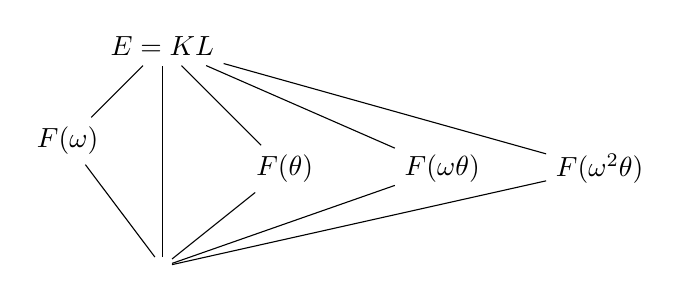
\begin{tikzpicture}[node distance = 2cm, auto]
                \node (E) {$E=KL$};
                \node (L) [below left of=E, node distance=1.7cm] {$F(\omega)$};
                \node (K) [below right of=E, node distance=2.2cm] {$F(\theta)$};
                \node (K1) [right of=K] {$F(\omega\theta)$};
                \node (K2) [right of=K1] {$F(\omega^2\theta)$};
                \node (Q) [below of=E, node distance=2.8cm] {$\Q$};
                \draw[-] (Q) to node {} (E);
                \draw[-] (Q) to node {} (K);
                \draw[-] (Q) to node {} (K1);
                \draw[-] (Q) to node {} (K2);
                \draw[-] (Q) to node {} (L);
                \draw[-] (E) to node {} (K);
                \draw[-] (E) to node {} (K1);
                \draw[-] (E) to node {} (K2);
                \draw[-] (L) to node {} (E);
            \end{tikzpicture}
        \end{center}
        \caption{Subfields of $E=KL$}
    \end{figure}

    The connection between these subfields is explained by Galois theory. We will be spending a lot of time on Galois theory.

    \begin{thm}
        Splitting fields are unique up to isomorphism. If $f \in F[x]$, and $E,E'$ are two splitting fields, then there exists an isomorphism $E \rightarrow E'$ that fixes $F$.
    \end{thm}

    We need a more general theorem:

    \begin{thm}
        Let $\varphi:F \rightarrow F'$ be an isomorphism of fields. Let $f \in F[x]$ and $f' \in F'[x]$ be its image under $\varphi$. Let $E/F$ be a splitting field for $f$ and $E'/F'$ be a splitting field for $f'$. Then $\varphi$ extends to an isomorphism $\sigma: E \rightarrow E'$.
        \begin{proof}
            Let $n = \mathrm{deg}f$. If $f$ splits already in $F[x]$, then $f'$ does over $F'$, so this case is trivial. Now assume the result for all $f$ with degree less than $n$.

            Let $p(x)$ be an irreducible factor of $f(x)$ of degree at least $2$ and $p'$ be the corresponding factor of $f'$. Let $\alpha \in E$ be a root of $p$ and $\beta \in E'$ a root of $p'$. Then there exists an isomorphism $\sigma':F(\alpha) \rightarrow F'(\beta)$ (remember that $F(\alpha) \simeq F[x]/(p(x)) \simeq F'[x]/(p'(x)) \simeq F'(\beta)$). Now we let $F_1 = F(\alpha)$ and $F_1' = F'(\beta)$, so we obtain the following commutative diagram:

            \begin{center}
                \begin{tikzcd}
                    E & E' \\
                    F_1 \arrow[hookrightarrow]{u} \arrow{r}{\sigma'} & F_1' \arrow[hookrightarrow]{u} \\
                    F \arrow[hookrightarrow]{u} \arrow{r}{\varphi} & F' \arrow[hookrightarrow]{u} \\
                \end{tikzcd}
            \end{center}
            By induction, we obtain an isomorphism $E \rightarrow E'$.
        \end{proof}
    \end{thm}

    ``It's better to have an example without a theorem than a theorem without an example.''

    \subsubsection{Algebraic Closure}

    \begin{defn}[Algebraic Closure]
        $\overline{F}/F$ is the algebraic closure of $F$ if every $f \in F[x]$ splits completely in $\overline{F}[x]$ and in no smaller extension and $\overline{F}/F$ is an algebraic extension.
    \end{defn}

    \begin{defn}[Algebraically Closed]
        If every $f \in K[x]$ has at least one root in $K$, then $K$ is algebraically closed field.
    \end{defn}

    \begin{exm}
        $\C$ is algebraically closed but is not the algebraic closure of $\Q$.
    \end{exm}

    Our goal is to prove that every field has a unique algebraic closure. First we will show that every field is contained in an algebraically closed field and then we will take the smallesy subfield of $K$ satisfying the definnition.

    \begin{prop}
        If $\overline{F}/F$ is an algebraic closure, then $\overline{F}$ is algebraically closed.
    \end{prop}

    \begin{lem}
        If $E/K$ and $K/F$ are algebraic, then $E/F$ is algebraic.
    \end{lem}

    ``If you take nothing from this lecture besides the fact that I have terrible sweater-shirt combinations, it should be that the quotient of a ring by a maximal ideal is always a field.''
    
    \begin{thm}
        Given any $F$, there exists an algebraically closed field containing $F$.\footnote{This is proven in the next lecture.}
    \end{thm}

    \subsection{Lecture 4 (Jan 31)}
    \subsubsection{Algebraic Closure Continued}

    Recall the definitions of algebraically closed and algebraic closure from last time. We continue the proof of Theorem 54 from last time.

    \begin{proof}[Proof of Theorem 54]
        Build $K$ as a union of fields $F \subset K_1 \subset K_2 \subset \cdots$ with $K = \cup_i K_i$. Let $R = F[\ldots, x_f, \ldots]$, which is a polynomial ring with a variable $x_f$ for each monic, nonconstant $f \in F[x]$. Let $I$ be the ideal generated by $f(x_f)$ for all nonconstant monic $f$. We show this is a proper ideal. If not, then there exists an expression $\sum_i g_i f_i(x_{f_i}) = 1$. Passing to a finite extension $F'/F$ such that each $f_i$ has a root in $F$. Then this implies that $0=1$. 
        
        Now let $M \supset I$ be a maximal ideal and $K_1 = R/m$. Then every monic nonconstant polynomial has a root in $K_1$. $K_1$ may not be algebraically closed, so continue to form a tower of fields, and then let $K$ be their union. We claim that $K$ is algebraically closed. To see this, observe that every $f \in K[x]$ lives in $K_i[x]$ for some $i$. Then $f$ has a root in $K_{i+1}$, so it has a root in $K$.
    \end{proof}

    \begin{cor}
        Let $F$ be a field and $K \supset F$ be algebraically closed. Let $\overline{F} \subset K$ be $\overline{F} = \Set{\alpha | \alpha \text{ alg/}F}$. Then $\overline{F}$ is the algebraic closure of $F$.

        \begin{proof}
            Let $f \in F[x]$. Then $f = \prod(x-\alpha_i)$ where each $\alpha_i \in K$. In fact, each $\alpha_i \in \overline{F}$ because it is algebraic.
        \end{proof}
    \end{cor}

    \begin{thm}
        Let $F$ be a field. Then the algebraic closure $\overline{F}/F$ is unique up to isomorphism.\footnote{The proof of this is not given in the book and will not be given here.}
    \end{thm}

    \subsubsection{(In)separability} 
    An intuitive way of thinking about this is that separable is nice and inseparable is not nice. Separable always happen in characteristic zero, but does not always happen in positive characteristics. Paul briefly mentioned the number field-function field analogy.

    Let $F$ be a field and $E$ be the splitting field of $f \in F[x]$. In $E$ we get a factorization $f = a_n \prod (x-\alpha_i)^{r_i}$. Then $\alpha$ is a simple root if it has multiplicity $1$ and is a multiple root otherwise. 

    \begin{defn}
        A polynomial $f \in F[x]$ is separable if it has no multiple roots in the splitting field $E/F$ of $f$.
    \end{defn}

    \begin{exm}
        Consider $f(x)= x^2-2 \in \Q[x]$. Then the splitting field is $\Q[\sqrt{2}]$ and $f$ is separable. 
        
        Consider $x^2+x+1 \in \F_2[x]$. This splits in $\F_4$ as $x^2+x+1 = (x - \theta)(x-(1+\theta))$, so it is separable. 
    \end{exm}

    \begin{exm}
        Consider the polynomial $x^2-t \in \F_2(t)[x]$. Then this polynomial is inseparable (this is because $\sqrt{t} = -\sqrt{t}$).
    \end{exm}

    How can we check for multiple roots? We take the formal derivative. ``We aren't doing calculus here, but polynomials are really all we do in calculus class anyway.'' We define an operator $D_x: F[x] \rightarrow F[x]$ that sends a polynomial to its formal derivative. Then this operator satisfies the usual linearity and product rules.

    \begin{prop}
        $\alpha$ is a multiple root of $f$ if and only if it is also a root of $D_x f$. In particular, the minimal polynomial of $\alpha$ divides both $f,D_x f$. Thus $f$ is separable if and only if it is coprime with $D_xf$.
        \begin{proof}
            Write $f = (x - \alpha)^ng(x)$ and differentiate.
        \end{proof}
    \end{prop}

    \begin{exm}
        $f(x) = x^n - 1$ is separable in characteristic $0$ because it is coprime to $D_xf = nx^{n-1}$. In positive characteristic, if $p \not\vert n$, $f$ is separable. Otherwise if $p | n$, then the derivative is zero and every root is a multiple root.
    \end{exm}

    \begin{exm}
        Consider $f = x^{p^n}-x \in \F_p[x]$. Then $D_xf = -1$, so there are no roots of $D_xf$ and $f$ is separable.
    \end{exm}

    \begin{prop}
        Let $\mathrm{char} F = 0$. Then any irreducible $f$ over $F$ is separable.
        \begin{proof}
            Suppose $\mathrm{deg} f = n$. Then the degree of $D_xf$ is $-1$. But then $f$ is irreducible, so it must be coprime to $D_xf$.
        \end{proof}
    \end{prop}

    \begin{rmk}
        Proposition 63 is false in general in positive characteristic, but is true for finite fields. This allows us to distinguish finite fields and infinite fields of positive characteristic.\footnote{the thing that allows us to distinguish finite fields is important in number theory and geometry.}
    \end{rmk}

    \begin{prop}
        Let $F$ be of characteristic $p$. Then the Frobenius endomorphism is injective.
        \begin{proof}
            It fixes $1$, so it must be injective.
        \end{proof}
    \end{prop}

    \begin{cor}
        The Frobenius endomorphism is an automorphism for any finite field $F$.\footnote{This generates the Galois group of $F/\F_p$.} In fact, every element of $F$ is a $p$-th power.
    \end{cor}

    \begin{defn}[Perfect Field]
        $K$ is a perfect field if either $\mathrm{char}\ K = 0$ or if every element of $K$ is a $p$-th power, where $p = \mathrm{char}\ K$. 
    \end{defn}

    \begin{prop}
        Every irreducible polynomial over a perfect field is separable.\footnote{We defer proof of this to next time. This is important for reasons of Galois theory.}
    \end{prop}

    \subsection{Lecture 5 (Feb 5)}
    
    \subsubsection{(In)separability Continued}

    Recall the definition of a perfect field and a separable extension.

    \begin{proof}[Proof of proposition 68]
        Assume that $f$ is irreducible of degree $n$. Then consider $\mathrm{gcd}(f, D_xf)$. It can happen that $\mathrm{deg}D_xf < n-1$. If we want $\mathrm{gcd}(f, D_xf) \neq 1$, then $D_xf = 0$. Therefore $f = g(x^p)$ for some $g \in K[x]$. Becuase $K$ is perfect, every coefficient of $g$ is a $p$-th power, which means that $f$ must be a $p$-th power, so it is not irreducible.
    \end{proof}

    \subsubsection{Classification of Finite Fields}

    We will classify finite fields. Consider the splitting field $E$ of $x^{p^n}-x$. This polynomial is separable, so $E$ must contains exactly $p^n$ roots. This forms a subfield of $E$ (just check the field axioms). Therefore, $E$ must be exactly the roots of $x^{p^n}-x$ and has order $p^n$, so $[E:\F_p] = n$. Therefore there exists a finite field of order any prime power.

    \begin{rmk}
        $E \simeq \F_p[x]/(f)$ where $f$ is irreducible. We can show by a counting argument that such $f$ exist for all $p,n$.
    \end{rmk}

    However, note that $x^{p^n}-x$ splits completely over any finite field of order $p^{n}$ (order of the group of units is $p^n-1$). Therefore, finite fields are unique.

    \begin{rmk}
        \begin{enumerate}
            \item We can perform the same construction starting with $\F_q$ for any prime power $q$.
            \item We can also show that $E^*$ is cyclic.
            \item Any finite division ring is a field.
        \end{enumerate}
    \end{rmk}

    \begin{prop}
        Suppose $f(x) \in F[x]$ is irreducible and that $F$ has characteristic $p$. Then there exists a unique $k \geq 0$ and a unique irreducible polynomial $f_{sep}(x)$ such that $p(x) = p_{set}(x^{p^k})$.

        \begin{proof}
            If $f$ is separable, then $f_{sep} = f$ and $k=0$. Otherwise, the derivative is zero and $f(x) = f_1(x^p)$. Then if $f_1$ is separable, $k=1$ and $f_{sep} = f_1$. If not, we can continue. However, by well-ordering, this process must terminate with $f = f_k(x^{p^k})$. Now we show that $f_k$ is irreducible. If not, then $f$ cannot also be irreducible (just replace $x$ with $x^{p^k}$ in any factorization).
        \end{proof}
    \end{prop}

    \begin{rmk}
        $f_{sep}, k$ are uniquely determined.
    \end{rmk}

    \begin{defn}[(In)separable Degree]
        The separable degree $\mathrm{deg}_s p(x) = \deg p_{sep}$ and the inseparable degree $\deg_i p(x) = p^k$. 
    \end{defn}

    We see that $\deg p = \deg_s p \cdot \deg_i p$. Observe that $p$ is separable if and only if $\deg_s p = \deg p$.

    \begin{defn}[Purely Inseparable]
        $p$ is purely inseparable if $\deg_s p = 1$.
    \end{defn}

    \begin{defn}[Separable Extension]
        An algebraic extension is separable if all elements are roots of separable polynomials. Otherwise, the extension is inseparable.
    \end{defn}

    Note that if $F$ is perfect, then all algebraic extensions are separable. In general, given $E/F$ algebraic, there exists a subfield $F \subset E_{sep} \subset E$ such that $E_{sep}/F$ is the largest separable extension of $F$ in $E$. If $E = F[x]/(f)$, then $E_{sep}$ has degree $\deg_s f$. The extension $E/E_{sep}$ is called purely inseparable.

    \begin{exm}
        Consider the field $F = \F_2(t)$. Let $f = x^2-t$ and $E = F[x]/(f)$. Note that $f(x) = f_{sep}(x^2)$, where $f_{sep} = x-t$. Thus $E/F$ is purely inseparable.
    \end{exm}

    \begin{exm}
        Again let $F = \F_2(t)$. Let $f = x^4+tx^2+t$. By Eisenstein, this polynomial is irreducible. Then note $f(x) = f_{sep}(x^2)$ where $f_{sep} = x^2+tx+t$. Then $[E:E_{sep}] = [E_{sep}:F] = 2$.
    \end{exm}

    \subsubsection{Cyclotomic Fields}

    Fix $n$. Then consider $\zeta_n = e^{2\pi i/n} \in \C$, which is algebraic ove $\Q$. Let $\Q(\zeta_n)/\Q$ be the subfield of $\C$ containing $\Q$ and $e^{2\pi i/n}$ is the primitive $n$-th root of unity. We want to write $\Q(\zeta_n) = \Q[x]/(\Phi_n(x))$.

    We will define a polynomial $\Phi_n$ and show that $\Phi_n | x^n-1$, $\Phi_n \in \Z[x]$, $\Phi_n$ is irreducible, and $\deg \Phi_n = \varphi(n)$.

    Define $\mu_n \subset \C$ be the group of all $n$-th roots of unity. Then clearly $\mu_n$ is cyclic generated by $\zeta$. If $d|n$, then $\mu_d < \mu_n$ generated by $\zeta^{n/d}$. The other primitive $n$-th roots are $P = \Set{\zeta^a | \mathrm{gcd}(a,n) = 1}$. Then $x^n-1 = \prod_{\omega \in \mu_n} (x - \omega)$. Define $\Phi_n(x) = \prod_{\omega \in P} (x - \omega)$. Observe that $x^n-1 = \prod_{d|n} \Phi_d(x)$. By construction, the first and fourth properties are true.

    \subsection{Lecture 6 (Feb 7)}
    \subsubsection{Cyclotomic Fields Wrap-up}
    Consider $\Q(\zeta_n)$ and recall the definition of the cyclotomic polynomial.

    \begin{thm}
        $\Phi_n(x) \in \Z[x]$ is irreducible with degree $\varphi(n)$.
        \begin{proof}
            We proceed using induction. Suppose $\Phi_m \in \Z[x]$ for all $1 \leq m < n$. Write $x^n-1 = f(x) \Phi_n(x)$. Then $f(x) \in \Z[x]$ and divides $x^n-1$ over $\Q$. Thus $\Phi_n \in \Q[x]$. Then by Gauss's lemma, $\Phi_n \in \Z[x]$.

            To show that $\Phi_n$ is irreducible, assume not and write $\Phi_n = f(x) g(x)$ where $f$ is irreducible. Let $\zeta$ be a primitive root that is a root of $f$ and choose $p \nmid n$, so $\zeta^p$ is also a primitive root. Then suppose $g(\zeta^p) = 0$, so $g(x^p)$ is divisible by $f$. Then we work mod $p$ and see that $(\overline{g}(x))^p\overline{g}(x^p) = \overline{f}(x)\overline{h}(x)$, so $\overline{f}$ and $\overline{g}$ have a common factor in $\F_p[x]$ and thus $\Phi_n$ has a multiple root mod $p$. However, this is not possible when $p \nmid n$. Therefore $\zeta^p$ is a root of $f$ and similarly, $\zeta^a$ is a root for any $a$ coprime to $n$. Thus $\Phi_n = f$.
        \end{proof}
    \end{thm}

    \section{Galois Theory}

    \subsection{Lecture 6 (cont.)}

    \subsubsection{Basics}
    The motivation behind Galois theory is to understand the structure of algebraic field extensions. Typical questions are:
    \begin{enumerate}
        \item What subfields $K \supset E \supset F$ can we have?
        \item Can we understand invariants of them?
        \item Suppose we have $K \supsetneq E \supsetneq F$. Can we construct it?
    \end{enumerate}

    Our main tool for studying these questions is group theory.

    \begin{defn}[Galois Group]
        Let $K/F$ be an extension. Then $\mathrm{Aut}(K/F)$ is the group of automorphisms of $K$ that fix $F$ pointwise.
    \end{defn}

    \begin{exm}
        $\Aut{\C/\R} \simeq \Z/2\Z$ and similarly for $\Q(\sqrt{D})/\Q$.
    \end{exm}
    \begin{exm}
        Let $\theta$ a root of $x^3+x^2-3x-1$. Then we see that the automorphism group is isomorphic to $\Z/3\Z$ generated by $\theta \mapsto \theta^2 - 2$.
    \end{exm}
    \begin{exm}
        The automorphism group of $\Q[x]/(x^3-2)$ is trivial.
    \end{exm}
    \begin{exm}
        The automorphism group of $\F_{p^n}/\F_p$ is isomorphic to $\Z/n/Z$ generated by the Frobenius endomorphism.
    \end{exm}
    \begin{exm}
        Let $E/\Q$ be the splitting field of $x^3-2$. Then we can show that $\Aut{E/\Q} \simeq S_3$.
    \end{exm}
    \begin{quest}[Inverse Galois Problem]
        Is every finite group the Galois group of an algebraic extension over the rationals?
    \end{quest}

    \begin{prop}
        Let $K/F$ be an extension with $\alpha \in K$ algebraic over $F$. Then if $\sigma \in \Aut{K/F}$, then $\sigma \alpha$ is a rot of the minimal polynomial of $\alpha$.
        \begin{proof}
            Let the minimal polynomial be $\sum a_ix^i$. Then $0 = \sigma \left( \sum a_i\alpha^i \right) = \sum \sigma(a_i\alpha^i) = \sum a_i (\sigma \alpha)^i$.
        \end{proof}
    \end{prop}

    \begin{cor}
        If $f \in F[x]$ is irreducible with roots in $K$, then $\Aut{K/F}$ must permute them.
    \end{cor}

    \begin{rmk}
        $\sigma$ may act trivially.
    \end{rmk}

    \subsubsection{Correspondences}

    Suppose $G = \Aut{K/F}$. Let $H \leq G$. Then $H$ determines a subset $K_H \subset K$ defined by the set of elements fixed by $H$.

    \begin{prop}
        $K_H$ is a subfield of $K$ containing $F$.
        \begin{proof}
            Left as an exercise to the reader.\footnote{Now I can write my own math textbook.}
        \end{proof}
    \end{prop}

    We can also produce a subgroup corresponding to each subfield. These correspondences are inclusion-reversing.

    \begin{thm}
        \begin{enumerate}
            \item If $H_1 \leq H_2$ then $K_{H_1} \supset K_{H_2}$.
            \item Of $E_1 \subset E_2$ then $\Aut{K/E_1} \geq \Aut{K/E_2}$.
        \end{enumerate}
    \end{thm}

    The proof of this theorem is straightforward. Ultimately, we will identify a class of ``Galois extensions'' for which these correspondences behave optimally.

    \begin{defn}[Galois Extension]
        Let $K/F$ be a finite extension. Then $K$ is a Galois extension of $F$ if $\abs*{\Aut{K/F}} = [K:F]$.
    \end{defn}

    \begin{exm}
        Quadratic extensions of $\Q$ are Galois. So are the extensions $\Q[x]/(x^3+x^2-2x-1)$ of $\Q$ and $\F_{p^n}/\F_p$.
    \end{exm}

    \begin{exm}
        The extension $\Q[x]/(x^3-2)$ is not Galois and neither is $E/\F_2(t)$ where $E = \F_2(t)[x]/(x^2-t)$.
    \end{exm}

    \begin{exm}
        Splitting fields of separable irreducible polynomials are Galois extensions. Thus the splitting field of any irreducible polynomial over a perfect field is Galois. Conversely, any Galois extension is the splitting field of a separable polynomial.
    \end{exm}

    \begin{prop}
        Let $E/F$ be the splitting field of a polynomial $f \in F[x]$. Then $\abs*{\Aut{E/F}} \leq [E:F]$ and equality holds if $f$ is separable.
    \end{prop}

    \subsection{Lecture 7 (Feb 12)}

    \subsubsection{Correspondences Continued}
    Last time, we discussed correspondences between subgroups of $G$ and fields between $K$ and $F$.

    We will prove Proposition 95.
    \begin{proof}[Proof of Proposition 95]
        Recall the proof of the uniqueness of splitting fields. We had this commutative diagram:
        \begin{center}
            \begin{tikzcd}
                E \arrow{r}{\sigma} & E' \\
                F \arrow[hookrightarrow]{u} \arrow{r}{\varphi} & F' \arrow[hookrightarrow]{u}
            \end{tikzcd}
        \end{center}
        We will show that the number of suitable $\sigma$ is at most $[E:F]$. We use induction. Then the number of extensions is $1$. Then let $p$ be an irreducible factor of $f$ of degree greater than $1$. Then let $p'$ be the corresponding factor of $f'$. Let $\alpha$ be a root of $p$. Then $F \subset F(\alpha) \subset E$. Then if $\sigma$ is any isomorphism, we can restrict to an isomorphism $\tau:F(\alpha) \simeq F'(\beta)$. Then the following diagram commutes.
        \begin{center}
            \begin{tikzcd}
                E \arrow{r}{\sigma} & E' \\
                F(\alpha) \arrow[hookrightarrow]{u} \arrow{r}{\tau} & F'(\beta) \arrow[hookrightarrow]{u} \\
                F \arrow[hookrightarrow]{u} \arrow{r}{\varphi} & F' \arrow[hookrightarrow]{u} \\
            \end{tikzcd}
        \end{center}
        Conversely, given any root $\beta$ of $p'$, we can make such a diagram. Then $\# \tau$ is at most $[F(\alpha):F]$. Use induction on the top half of the diagram and the result follows. 
    \end{proof}

    Eventually we see that $K/F$ is Galois if and only if it is a splitting field of a separable polynomial.

    \begin{exm}
        Consider $\Q(\sqrt{D})/\Q$ for $D \in \Z$ squarefre. Then $\sqrt{D} \mapsto - \sqrt{D}$ is an automorphism and the Galois group of this extension is $\Z/2\Z$.
    \end{exm}

    \begin{exm}
        Consider the field $\Q(\sqrt{2}, \sqrt{3})$. Then the automorphisms $\sqrt{2} \mapsto -\sqrt{2}$ and $\sqrt{3} \mapsto -\sqrt{3}$ are nontrivial and have order $2$. Thus the Galois group is $(\Z/2\Z)^2$. Here is the subfield lattice.
        \begin{center}
            \begin{tikzpicture}[node distance = 2cm, auto]
                \node (E) {$\Q(\sqrt{2}, \sqrt{3})$};
                \node (L) [below of=E] {$\Q(\sqrt{6})$};
                \node (K1) [right of=L] {$\Q(\sqrt{2})$};
                \node (K2) [left of=L] {$\Q(\sqrt{3})$};
                \node (Q) [below of=L] {$\Q$};
                \draw[-] (Q) to node {} (L);
                \draw[-] (L) to node {} (E);
                \draw[-] (Q) to node {} (K1);
                \draw[-] (Q) to node {} (K2);
                \draw[-] (E) to node {} (K);
                \draw[-] (E) to node {} (K1);
                \draw[-] (E) to node {} (K2);
            \end{tikzpicture}
        \end{center}
        Here is the subgroup lattice:
        \begin{center}
            \begin{tikzpicture}[node distance = 2cm, auto]
                \node (E) {$1$};
                \node (L) [below of=E] {$\gen{\sigma\tau}$};
                \node (K1) [right of=L] {$\gen{\sigma}$};
                \node (K2) [left of=L] {$\gen{\tau}$};
                \node (Q) [below of=L] {$(\Z/2\Z)^2$};
                \draw[-] (Q) to node {} (L);
                \draw[-] (L) to node {} (E);
                \draw[-] (Q) to node {} (K1);
                \draw[-] (Q) to node {} (K2);
                \draw[-] (E) to node {} (K);
                \draw[-] (E) to node {} (K1);
                \draw[-] (E) to node {} (K2);
            \end{tikzpicture}
        \end{center}
    \end{exm}

    \begin{exm}
        Recall the splitting field of $x^3-2 = f$. Let $\theta$ be a root of $f$ and $\omega$ be a root of $\Phi_3$. Then $E = \Q(\omega, \theta)$. The total degree of this extension is $6$ and thus $\Aut{(E/F)} = 6$. But then note that $\sigma$ that sends $\theta \mapsto \omega\theta$ is of order $3$, while $\tau$ that sends $\omega \mapsto \omega^2$. However, $\sigma\tau \neq \tau\sigma$, so the automorphism group is $S_3$. The subfield lattice is somewhere earlier in the notes, so I will just include the subgroup lattice:
        \begin{center}
            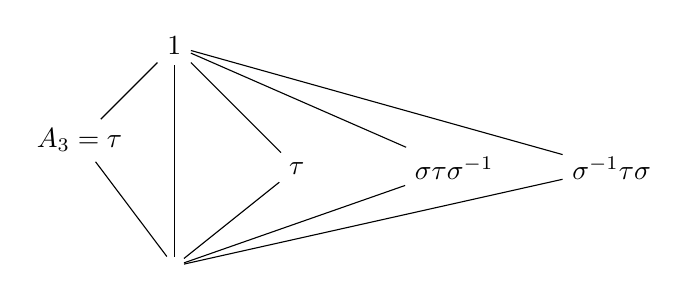
\begin{tikzpicture}[node distance = 2cm, auto]
                \node (E) {$1$};
                \node (L) [below left of=E, node distance=1.7cm] {$A_3 = \gen{\tau}$};
                \node (K) [below right of=E, node distance=2.2cm] {$\gen{\tau}$};
                \node (K1) [right of=K] {$\gen{\sigma\tau\sigma^{-1}}$};
                \node (K2) [right of=K1] {$\gen{\sigma^{-1}\tau\sigma}$};
                \node (Q) [below of=E, node distance=2.8cm] {$\Q$};
                \draw[-] (Q) to node {} (E);
                \draw[-] (Q) to node {} (K);
                \draw[-] (Q) to node {} (K1);
                \draw[-] (Q) to node {} (K2);
                \draw[-] (Q) to node {} (L);
                \draw[-] (E) to node {} (K);
                \draw[-] (E) to node {} (K1);
                \draw[-] (E) to node {} (K2);
                \draw[-] (L) to node {} (E);
            \end{tikzpicture}
        \end{center}
    \end{exm}

    \begin{rmk}
        Automorphisms in the previous example that act on $\Q(\omega)$ take it to itself while automorphisms that are nontrivial on the $\Q(\theta)$ do not preserve it. We will see that this is because $A_3$ is a normal subgroup of $S_3$ but $\Z/2\Z$ is not.
    \end{rmk}

    Our goal now is to prove the fundamental theorem of Galois theory. The idea is a complete characterization of the subgroup and subfield lattices. Today we will prove some of the technical results that we need.

    \begin{defn}[Character]
        Let $G$ be a group and $L$ a field. Then a character $\chi$ of $G$ with values in $L$ is a homomorphism of groups $\chi: G \rightarrow L^{\times}$ (Note that this is completely governed by the abelianization of the group).
    \end{defn}

    \begin{defn}[Linear independence]
        A collection $\chi_1, \ldots, \chi_n$ is linearly independent if there does not exist a linear relation $\sum a_i \chi_i = 0$ where $a_i \in L$ and the $a_i$ are not all $0$.
    \end{defn}

    \begin{exm}
        Let $G = \C^{\times} \times \C^{\times}$. Then we see that $\chi_1(a,b) = ab$ and $\chi_2(a,b) = a/b$ are linearly independent (if not, then $b^2$ is constant for all $b \in \C$).
    \end{exm}

    \begin{rmk}
        Any character\footnote{Well, any algebraic character. For example, complex conjugation is an automorphism of $\C^{\times}$ that is not algebraic.} of $G$ is of the form $\chi(a,b) = a^nb^m$ for some fixed $n,m \in \Z$ and any finite subset if linearly independent.
    \end{rmk}

    \begin{thm}
        Any finite subset of distinct characters $\chi_1, \ldots, \chi_n$ is linearly independent.
        \begin{proof}
            Take a minimal relation of the form $a_1 \chi_1 + \cdots + a_m\chi_m = 0$ where all $a_i \neq 0$. Then for all $g \in G$, we have $a_1\chi_1(g) + \cdots + a_m\chi_m(g) = 0$. Then there exists $g_0 \in G$ such that $\chi_1(g_0) \neq \chi_m(g_0)$. Therefore, for all $g \in G$, $a_1\chi_1(g_0g) + \cdots + a_m\chi_m(g_0g) = 0$.

            Thus, $a_1\chi_1(g_0)\chi_1(g) + \cdots + a_m\chi_m(g_0)\chi_m(g) = 0$. Then we must have $\sum_{i=2}^m a_i(\chi_i(g_0) - \chi_i(g_0))\chi_i(g) = 0$ for all $g\in G$. But this is a shorter length expression with not all coefficients zero, which contradicts minimality of the original relation.
        \end{proof}
    \end{thm}

    If we have a field homomorphism $\sigma: K \hookrightarrow L$, then this gives a character of $K^{\times}$.

    \begin{cor}
        Any distinct field embeddings are linearly independent.
    \end{cor}

    \begin{cor}
        Distinct automorphisms of a field are linearly independent.
    \end{cor}

    \subsection{Lecture 8 (Feb 14 $\heartsuit$)}
    \subsubsection{Towards the Fundamental Theorem of Galois Theory}

    Our goal is to prove the Fundamental Theorem of Galois Theory. Recall the definition of a character and that any finite set of distinct characters is linearly independent. In particular, note that a collection of distinct field embeddings is linearly independent.

    Now suppose $K = L$. Then any finite set of automorphisms is linearly independent.

    \begin{thm}
        Let $G = \{\sigma_i \mid 1 \leq i \leq n\}$ be a subgroup of $\Aut{K}$. Let $F \subset K$ be the fixed field. Then $[K:F] = \abs{G} = n$.
        \begin{proof}
            First suppose that $n > [K:F] = m$. Then let $\omega_1, \ldots, \omega_m$ be an $F$-basis of $K$. Consider the linear system \[\sum_{i=1}^n \sigma_i(\omega_j) \chi_i = 0,\] where $j = 1, \ldots, m$. Because there are fewer euqations than variables, there exists a non-trivial solution $(\beta_1, \ldots, \beta_n) \in K^n$. Choose $m$ arbitrary elements $a_1, \ldots, a_m \in F$. Then $\sigma_i(a_k) = a_k$ for all $i$. In the linear system multiply the $j$th equation by $a_j$ and substitute $\chi_i \gets \beta_i$.

            Now we have the linear system $\sum_{i=1}^n \sigma_i(a_j \omega_j) \beta_i = 0$. Adding the equations together, we obtain \[\sum_{i=1}^n \sigma_i \left(\sum_{j=1}^m a_j \omega_j \right) \beta_i = 0.\] Because the $a_j$ are arbitrary, then we can put any element of $K$ inside the $\sigma_i$. Therefore $\sum_{i=1}^n \sigma_i(k) \beta_i = 0$ for all $k \in K$, which is a nontrivial linear dependence on the $\sigma_i$, which is impossible.

            Now we suppose that $n < [K:F]$. Then choose $\alpha_1, \ldots, \alpha_{n+1}$ linearly independent over $F$ and form a linear system \[\sum_{i=1}^{n+1} \sigma_j(\alpha_i) \chi_i = 0,\] where $j = 1, \ldots, n$. There is a nontrivial solution, so let $(\beta_1, \ldots, \beta_{n+1})$ be the solution. We claim that at least one $\beta_i$ is in $K\setminus F$ (otherwise we have a linear dependence of the $\alpha_i$ using the $\beta_i$ as coefficients).  Now choose a solution with a minimum number of nonzero elements, say $r \leq n+1$. We can assume that $\beta_r = 1$.

            We will form a new nontrivial solution with fewer nonzero elements. Assume without loss of generality that $\beta_1 \not\in F$. Then the system becomes \[\sigma_j(\alpha_r) + \sum_{i=1}^{r-1} \sigma_j(\alpha_i) \beta_i = 0.\] We will choose $\sigma' \in G$ such that $\sigma'(\beta_1) \neq \beta_1$. Then note that left multiplication by $\sigma'$ permutes the $\sigma_i$. Therefore, we apply $\sigma'$ to our system and renumber. We now have the system \[\sigma_j(\alpha_r) + \sum_{i=1}^{r-1} \sigma_j(\alpha_i) \sigma'(\beta_i) = 0.\] Taking the difference of our two systems, we have the new equation \[\sigma_j(\alpha_1)(\beta_1 - \sigma'(\beta_1)) + \cdots + \sigma_j(\alpha_{r-1})(\beta_{r-1} - \sigma'(\beta_{r-1})) = 0.\] Because the first coefficient is nonzero, we now have a nontrivial solution with fewer nonzero elements.
        \end{proof}
    \end{thm}

    \begin{cor}
        If $K/F$ is finite, then $\abs{\Aut{K/F}} \leq [K:F]$. Then equality happens if and only if $F$ is the fixed field of $\Aut{K/F}$.
        \begin{proof}
            Let $F'$ be the fixed field. Then by the theorem, $[K:F'] = \abs{\Aut{K/F}}$. The desired result holds by multiplicativity.
        \end{proof}
    \end{cor}
    
    \begin{cor}
        Let $G$ be a finite group of automorphisms of $K$ with fixed field $F$. Then $\Aut{K/F} = G$ and $K/F$ is a Galois extension with Galois group $G$.
        \begin{proof}
            Our assumptions imply that $G \leq \Aut{K/F}$ and $\abs{G} \leq \Aut{K/F}$. Then recall that $\abs{\Aut{K/F}} \leq [K:F]$. Therefore $[K:F] = \abs{G} \leq \abs{\Aut{K/F}} \leq [K:F]$, so they are all equal.
        \end{proof}
    \end{cor}

    \begin{cor}
        Let $G_1 \neq G_2$ be distinct subgroups of $\Aut{K}$. Let $F_1,F_2$ be the fixed fields. Then $F_1 \neq F_2$.
        \begin{proof}
            Suppose $F_1 = F_2$. Then $G_2$ fixes $F_1$, so $G_2 \leq G_1$. Similarly, $G_1 \leq G_2$. Thus they are equal.
        \end{proof}
    \end{cor}

    The consequence of these is that taking fixed fields of different subgroups of $\Aut{K}$ gives different subfields of $K$ over which $K$ is Galois.

    \begin{thm}
        $K/F$ is Galois if and only if $K$ is the splitting field of a separable polynomial over $F$. Furthermore, if this is true then any polynomial over $F$ with a root in $K$ is separable and has all its roots in $K$.
        \begin{proof}
            We already showed that Galois is implied by splitting field. Now assume $K/F$ is Galois. Then $G = \mathrm{Gal}(K/F) \coloneqq \Aut{K/F}$. Write $G = \{1, \sigma_2, \ldots, \sigma_n\}$. Let $p \in F[x]$ be irreducible with a root $\alpha \in K$. We show all the roots are in $K$. Consider the list $\{\alpha, \sigma_2 \alpha, \ldots, \sigma_n \alpha\}$. Assume the distinct elements in the orbit are $\alpha_1, \ldots, \alpha_r$. It must be that $f(x) = \prod_{i=1}^r (x-\alpha_i) \in F[x]$. Then $p$ is irreducible with root $\alpha$, so $p$ is the minimal polynomial of $\alpha$ over $F$. Then $p \mid f$ in $F[x]$. However, $f \mid p$ in $K[x]$. Therefore $p = f$ is separable and has all roots in $K$.

            Now we prove that $K/F$ is a splitting field. Assume $K/F$ is Galois with group $G$. Then choose $\omega_1, \ldots, \omega_n$ a basis of $F$ over $K$. Let $p_1, \ldots, p_n$ be the minimal polynomials over $F$ of the $\omega_i$. We know each is separable and has all its roots in $K$. Take $g$ to be the $\mathrm{LCM}$ of the $p_i$. We see that $g$ is squarefree, so it is separable. We see that $K$ is the splitting field. The roots are all in $K$, so the splitting field is a subfield. The $\omega_i$ are all roots of $g$, so the splitting field is $K$.
        \end{proof}
    \end{thm}

    We have seen that the following are equivalent:
    \begin{enumerate}
        \item $K$ is a Galois extension of $F$.
        \item $K$ is the splitting field of a separable polynomial in $F$;
        \item $K$ is an extension of $F$ such that $F$ is exactly the fixed field of $\Aut{K/F}$;
        \item $K$ is an extension of $F$ such that $[K:F] = \abs{\Aut{K/F}}$;
        \item $K$ is a finite, normal, and separable extension of $F$.
    \end{enumerate}

    \subsection{Lecture 9 (Feb 21)}%
    
    We will finally get to the Fundamental Theorem of Galois Theory.

    \begin{thm}
        Let $K/F$ be a Galois extension with group $G$. Then there is an inclusion-reversing bijection between subfields of $K$ containing $F$ and subgroups of $G$. This correspondence takes a subfield to the subgroup fixing it and a subgroup to its fixed field. The bijection satisfies
        \begin{enumerate}[label=(\alph*)]
            \item $[G:H] = [E_H:F]$ and $\abs{H} = [K:E_H]$;
            \item $K/E$ is Galois with group $H_E \leq G$;
            \item $E/F$ is Galois if and only if $H_E \trianglelefteq G$. In this case $\mathrm{Gal}(E/F) \simeq G/H_E$. Even if $H_E$ isn't normal, the isomorphisms of $E$ into an algebraic closure that fix $F$ are in bijection with the cosets.
            \item If $E_1, E_2$ correspond to $H_1,H_2$, then $E_1 \cap E_2$ corresponds to $(H_1, H_2)$ the subgroup generated by $H_1H_2$. The compositum $E_1E_2$ corresponds to the intersection $H_1 \cap H_2$. Therefore we have a correpondence between the subgroup lattice and the subfield lattice.
        \end{enumerate}
    \end{thm}

    An example is the lattices for the splitting field of $x^3-2$ over $\Q$. These are somewhere earlier in the notes. Note that we have proven most of this theorem already.

    \begin{proof}[Proof of Theorem 112]
        We have already shown most of this theorem. For example, we showed that the map from subgroups to subfields is injective. To see that is is surjective, choose a subfield $E$ and suppose $K/F$ is the splitting field of $f \in F[x]$. Then $K/E$ is Galois and $E$ is the fixed field of $\Aut{K/E} < G$.

        Now we will show (c). Suppose $E$ is the fixed field of $H \leq G$. Then for any $\sigma \in G$, take $E$ to $\sigma(E)$, isomorphic to $E$ fixing $F$. Let $\tau: E \to \tau(E)$ be an isomorphism in a fixed algebraic closure fixing $F$. Let $\alpha \in E$ have minimial polynomial $m_{\alpha}(x)$ over $F$. Then $\tau \alpha$ is another root of $m_{\alpha}$. If $K$ is the splitting field of $f \in F[x]$, then it is the splitting field of the same polynomial over $E$. Therefore it is the splitting field of $\tau f$ over $\tau(E)$. But $\tau f = f$. Then by the uniqueness of splitting fields, we have a commutative diagram: 
        \begin{center}
            \begin{tikzcd}
                K \arrow{r}{\sigma} & K' \\
                E \arrow[hookrightarrow]{u} \arrow{r}{\tau} & \tau(E) \arrow[hookrightarrow]{u} \\
                F \arrow[hookrightarrow]{u} \arrow{r}{\mathrm{id}} & F \arrow[hookrightarrow]{u} \\
            \end{tikzcd}
        \end{center}
        Therefore, any such $\tau$ comes from $\sigma \in G$. When do $\sigma, \sigma'$ give the same $\tau$? Then $\sigma^{-1}\sigma' = \mathrm{id}$, which happens if and only if $\sigma, \sigma'$ determine the same coset of $H$. Then the statement of normality follows. Part (d) is easy and is left to the treatment in D\&F.
    \end{proof}

        \subsubsection{Computing Galois Groups}%
        We use the following fact:
        \begin{prop}
            Let $f$ be irreducible of degree $n$. Then define $\Gal{f} \coloneqq \Gal{E/Q}$, where $E$ is the splitting field of $f$. Then $G = \Gal{f} \leq S_n$ and acts transitively.
        \end{prop}

        For example, if $n = 3$, then the only groups are $S_3,A_3$.
        \begin{exm}
            Let $f = x^3 + 7x+14$. Note that $f$ has only one real root (derivative is always positive). Therefore, the two complex roots are conjugate, so there is an element of order $2$ in the Galois group. Therefore, the Galois group of $f$ is $S_3$.
        \end{exm}

        \begin{exm}
            Let $F = \Q(\theta)$, where $\theta = \sqrt{2+\sqrt{2}}$. Note that $(\theta^2-2)^2 - 2 = 0$. Then our candidate polynomial is $f = x^4 - 4x^2+2$. This is irreducible by Eisenstein with roots $\pm \sqrt{2 \pm \sqrt{2}}$. We need to see whether $\sqrt{2-\sqrt{2}} \in F$. We see that $\sqrt{2} \in F$ and that $\sqrt{2+\sqrt{2}}\sqrt{2-\sqrt{2}} = \sqrt{2}$, so all roots are in $\Q(\theta)$. Therefore $F$ is the splitting field of $f$. Then we see that either $G = \Z/4\Z$ or $G = (\Z/2\Z)^2$. Then the automorphism $\sigma$ that takes $\theta \to \alpha$ has order $4$, so the group is $\Z/4\Z$.
        \end{exm}

        \begin{exm}
            Consider $f = x^6+3$. This is irreducible by Eisenstein. Then take $\alpha = \sqrt{3}$ and $\rho = e^{2 \pi i /12}$ a primitive twelfth root of unity.We see that the roots are $\rho\alpha, \ldots, \rho^{11}\alpha$. We determine if $\Q(r_1)$ is the splitting field. This is true if and only if the field contains $\rho^2$, which is true ($\sqrt{3} \cdot i = (\rho\alpha)^3$). Thus the extension has degree $6$ and is either $S_3$ or $\Z/6\Z$.
        \end{exm}

        \subsection{Lecture 10 (Feb 26)}
        There is an exam on March $7$ in the evening. Topics will be announced later.

        We finish the computation of the Galois group of $S_3$. Observe that complex conjugation is an automorphism of the extension. Then there exists another $\sigma$ that sends $r_1 \mapsto r_2$. This has order $2$, so the Galois group is $S_3$.

        Note that if we set $f = x^6+2$, then this problem becomes must harder.

        \begin{exm}
            Let $\theta = \sqrt{(2+\sqrt{2})(3+\sqrt{3})}$ and consider $K = \Q(\theta)$. Note that $\theta \notin \Q(\sqrt{2}, \sqrt{3})$.  Then we see that $K$ is the splitting field, so the Galois group $G$ has order $8$. $G$ must have at least three subgroups of order $4$, so it can only be $Q_8$ or $(\Z/2\Z)^2$. We can find an element of order $4$, however ($\sqrt{(2 + \sqrt{2})(3 + \sqrt{3})} \mapsto \sqrt{(2 - \sqrt{2})(3 + \sqrt{3})}$), so $G = Q_8$.
        \end{exm}

        Now if we try $\theta(a,b) = \sqrt{(a + \sqrt{a})(b + \sqrt{b})}$ with $a < b < 100$ prime, we get Galois groups:
        \begin{description}
            \item[$Q_8$] $(2,3), (2,19), (2,73)$;
            \item[$\Z/4\Z \times \Z/2\Z$]] $(2,5), (2,17), (2,37), (5.17), (5,37)$;
            \item[Order $16$] $(2,7), (2,11), (2,13)$;
            \item[Order $32$] $(3,11)$.
        \end{description}

        Note that the order $16$ group is the almost direct product of $Q_8, \Z/4\Z$. 

        \subsubsection{Finite Fields}
        Recall that we can construct $\F_{p^n}/\F_p$ for all $p,n$, which is Galois. We will show that $G$ is cyclic of order $n$.

        \begin{prop}
            $\mathrm{Gal}(\F_{p^n}/\F_p) \simeq \Z/n\Z$ and is generated by the Frobenius element.
            \begin{proof}
                Consider orders of the Frobenius element. This is left as an exercise to the reader.
            \end{proof}
        \end{prop}
        
        Now we can consider a subextension $\F_{p^n}/\F_{p^d}$ where $d | n$. This has Galois group $\Z/(n/z)\Z$.

        \begin{prop}
            $\F_{p^n}^{\times}$ is cyclic.
            \begin{proof}
                This is left as an exercise. Just consider the elements of order dividing $p^d-1$ for $d | n$.
            \end{proof}
        \end{prop}

        \begin{rmk}
            The fact about roots you need to prove the previous proposition leads to the Miller-Rabin primality test.
        \end{rmk}

        Now recall that $K/F$ is simple if it is generated by a primitive element.

        \begin{cor}
            $\F_{p^n}/\F_p$ is simple. This implies that there exists an irreducible polynomial of degree $n$ over $\F_p$.
            \begin{proof}
                Take a generator $\theta$ of the group of units. This generates the field extension.
            \end{proof}
        \end{cor}

        \begin{rmk}
            $x^{p^n} - x$ is the product of all irreducible polynomials of degree $d | n$. This will allow us to count the irreducible polynomials.
        \end{rmk}

        \subsection{Lecture 11 (Feb 28)}
        
        Last time we proved that all finite fields are simple extensions of $\F_p$. 

        \begin{exm}
            Let $p = 2$. Then $x^4-x = x(x+1)(x^2+x+1)$ and $x^8-x = x(x+1)(x^3+x+1)(x^3+x^2+1)$.
        \end{exm}

        To count irreducible polynomials over $\F^p$, we use M\"obius inversion. Recall the M\"obius function from number theory. Consider $F,f$ on the positive integers. Then suppose $F = \sum_{d|n} f(d)$.

        \begin{thm}[M\"obius Inversion]
            $f(n) = \sum_{d|n} \mu(d)F(n/d)$. 
        \end{thm}

        Let $\psi(n)$ be the number of irreducible polynomials of degree $n$ over $\F_p$. Then note that $p^n = \sum_{d|n} d\psi(d)$. Therefore, $n\psi(n) = \sum_{d|n}\mu(d)p^{n/d}$, so $\psi(n) = \frac{1}{n} \sum_{d|n} \mu(d)p^{n/d}$. We can prove that $\psi(n) \neq 0$, but it's not clear that it is an integer.

        Now we consider the algebraic closure $\overline{\F_p} = \bigcup_{n \geq 1} \F_{p^n}$, whic is infinite. Note that the subfields are ordered by divisibility.

        \subsubsection{Primitive Elements}

        Our goal is now the primitive element theorem:
        \begin{thm}
            If $K/F$ is finite and separable, then it is simple.
        \end{thm}

        \begin{prop}
            Suppose $K/F$ is Galois and let $F'/F$ be any extension. Then $KF'/F'$ is Galois with $\mathrm{Gal}(KF'/F') \simeq \mathrm{Gal}(K/K\cap F')$.
            \begin{proof}
                We see that $K$ is the splitting field of $f \in F[x]$. Then $f \in F'[x]$ and $KF'$ is the splitting field of $f \in F'[x]$. Thus $KF'/F'$ is Galois.

                Consider the map $\varphi: G(KF'/F') \to G(K/F)$ given by restriction. Then $\sigma$ fixes $F'$, so it fixes $F$. Note that the kernel is all $\sigma$ that restrict to the identity. Then $\sigma$ is the identity on $K$ and fixes $F'$ by construction, so is the identity on the composite. Therefore, $\varphi$ is injective. Let $K_H$ be the fixed field of the image. Then $K_H \supset K \cap F'$ However, it must be a subfield of $F'$, so it must be equal to $K \cap F'$.
            \end{proof}
        \end{prop}

        \begin{cor}
            $[KF':F] = \frac{[K:F][F':F]}{[K\cap F':F]}$.
            \begin{proof}
                We know that $[KF':F'] = [K:K\cap F']$, so
                \begin{align*}
                    [KF':F] &= [KF':F'][F':F] \\
                            &= [K:K\cap F'][F':F] \\
                            &= \frac{[K:F]}{[K \cap F':F]} [F':F].
                \end{align*}
            \end{proof}
        \end{cor}

        \begin{prop}
            Let $K_1, K_2$ be Galois extensions of $F$. Then $K_1 \cap K_2/F$ and $K_1K_2/F$ are Galois.
            The Galois group of $K_1K_2/F$ is \[H = \Set{(\sigma, \tau)| \sigma \in G(K_1/F), \tau \in G(K_2/F), \sigma|_{K_1\cap K_2} = \tau|_{K_1 \cap K_2}}.\]
            \begin{proof}
                Suppose $p \in F[x]$ is irreducible with a root in $K_1 \cap K_2$. Then all roots of $p$ are in both $K_1, K_2$, so $K_1 \cap K_2/F$ is finite, normal, and separable. Now suppose $K_i$ is the splitting field of separable polynomials $f_i$. Then $K_1K_2$ is the splitting field of the separable polynomial $\mathrm{LCM}(f_1, f_2)$, so it is Galois.

                Now consider the map $G(K_1K_2/F) \to G(K_1/F) \times G(K_2/F)$ given by the product of the restrictions. First we see that this is injective. This is because anything in the kernel is trivial on both $K_1, K_2$, so it is the identity on the composite. Clearly, the image is in $H$ because the restrictions of $\sigma$ to $K_1, K_2$ agree on $K_1 \cap K_2$. To find the order, we see that $\abs{H} = \frac{\abs{G(K_1/F)}\abs{G(K_2/F)}}{\abs{G(K_1\cap K_2 / F)}}$. On the other hand, $[K_1K_2:F] = [K_1K_2:K_1][K_1:K_1 \cap K_2][K_1 \cap K_2:F] = [K_2:K_1 \cap K_2][K_1:F] = \frac{[K_2:F]}{[K_1 \cap K_2:F]}[K_1:F]$.
            \end{proof}
        \end{prop}

        A partial converse is that if $G(K/F) \simeq G_1 \times G_2$, then $K = K_1K_2$ where $K_i$ is the fixed field of $G_i$.

        \begin{cor}
            Let $E/F$ be finite and separable. Then there exists a Galois extension $K \supset E \supset F$ such that any Galois extension of $F$ containing $E$ is an extension of $K$.
            \begin{proof}
                Take an $F$-basis $\alpha_1, \ldots, \alpha_k$ of $E$. Take their minimal polynomials and the composite of the splitting fields to take a Galois extension. Then take the intersection of all Galois extensions of $F$ containing $E$ to get the Galois closure.
            \end{proof}
        \end{cor}

        \begin{exm}
            $G(\Q(\sqrt{2}, \sqrt{3})) = (\Z/2\Z)^2$.
        \end{exm}

        \subsection{Lecture 12 (Mar 5)}
        
        The exam will be in LGRT $206$ from $7$-$8:30$ covering everything through section $14.2$.
        
        From last time, our goal is to prove the primitive element theorem.

        \begin{prop}
            Suppose $K/F$ is finite. Then $K = F(\theta)$ if and only if there are only finitely many intermediate fields $K \supset E \supset F$.
            \begin{proof}
                Let $K = F(\theta)$. Let $f$ be the minimal polynomial and $E$ be a subfield. Then let $g$ be the minimal polynomial of $\theta$ in $E[x]$. Clearly $g | f$ in $E[x]$. Let $E'/F$ be the field generated by the coefficients of $g$. Then $E' \subset E$ and the minimal polynomial of $\theta$ over $E'$ is still $g$. Therefore $[K:E] = [K:E']$, so $E = E'$. Therefore subfields of $K$ correspond to different monic fractions of $f$, of which there are only finitely many.

                Now we assume there are only finitely many intermediate fields. We may also assume $F$ is infinite. We show that a primitive element exists for $F(\alpha, \beta)$, which is sufficient by induction. Consider the fields $\{F(\alpha+c\beta) \mid c \in F\}$. Given that there are only finitely many intermediate fields, there exist $c,c' \in F$ such that $F(\alpha+c\beta) = F(\alpha+c'\beta)$. Then we see that $\alpha,\beta \in F(\alpha+c\beta)$, so $F(\alpha, \beta) = F(\alpha+c\beta)$.
            \end{proof}
        \end{prop}

        We will now prove the finite element theorem.
        \begin{proof}[Proof of Theorem 125]
            Take the Galois closure $K$ of $E/F$. Then $[K:F]$ is finite, which means there are only finitely many subfields between $K$ and $F$. In particular, there must be only finitely many subfields between $E$ and $F$. Now use the proposition.
        \end{proof}

        \subsubsection{Cyclotomic Fields}
        
        Let $\zeta_n$ be a primitive $n$th root of unity. Then recall the $n$th cyclotomic polynomial $\Phi_n(x) \in \Q[x]$, which is irreducible of degree $\phi(n)$.

        We will show that $\Q(\zeta_n)/\Q$ is Galois with $G \simeq (\Z/n\Z)^{\times}$. Define a morphism $(\Z/n/Z)^{\times} \to \mathrm{Gal}(\Q(\zeta_n)/\Q)$ given by $a \mapsto \sigma_a$. Analyzing this, we see that this is an isomorphism. Paul claims that this is not canonical.

        \begin{exm}
            Consider $\Q(\zeta_7)$. Then $G \simeq \Z/6\Z$. The subgroups have order $1,2,3,6$.
            Therefore the subgroup lattice is:
            \begin{center}
                \begin{tikzcd}
                    & \{0\} & \\
                    \Z/3\Z \arrow[dash]{ur} & & \Z/2/Z \arrow[dash]{ul} \\
                    & \Z/6/Z \arrow[dash]{ul} \arrow[dash]{ur}
                \end{tikzcd}
            \end{center}
            
            The subfield lattice is:
            \begin{center}
                \begin{tikzcd}
                    & \Q(\zeta_7) & \\
                    \Q(\sqrt{-7}) \arrow[dash]{ur} & & K = \Q[x]/(x^3+x^2-2x-1) \arrow[dash]{ul} \\
                    & \Z/6/Z \arrow[dash]{ul} \arrow[dash]{ur}
                \end{tikzcd}
            \end{center}
        \end{exm}
        
        Now suppose $p$ is an odd prime and let $H \leq G = (\Z/p\Z)^{\times}$. We can define $\alpha_H = \sum_{\sigma \in H} \sigma(\zeta_n)$. This is invariant under $H$ and generates the fixed field of $H$. Note that this does not in general because the primitive $n$th roots need not be linearly independent over $\Q$.

        \begin{exm}
            Let $p = 7$. Then note that $\Z/2\Z$ is generated by $\zeta \mapsto \zeta^6 = \overline{\zeta}$. Then the fixed field is clearly real. To find the generator, note that $(\zeta+\zeta^{-1})^3 = \zeta^3 + 3\zeta + 3 \zeta^{-1} + \zeta^{-3}, (\zeta+\zeta^{-1})^2 = \zeta^2+2+\zeta^{-2}$. Then recall that $\zeta + \zeta^2 + \zeta^3 + \zeta^{-1} + \zeta^{-2} + \zeta^{-3} = -1$. Using these facts, it is easy to see that $\zeta+\zeta^{-1}$ satisfies $x^3+x^2-2x-1$.

            Also, we can see that $\alpha_{\Z/3\Z} = \zeta + \zeta^2 + \zeta^4$. Then it is straightforward to find the minimal polynomial, which is quadratic of discriminant $-7$.
        \end{exm}

        Now recall that $\phi$ is multiplicative. Then we will see that $\Q(\zeta_n)$ is the compositum of the $\Q(\zeta_{p_i^{e_i}})$.

        \begin{thm}[Kronecker-Weber]
            If $F/\Q$ is Galois with abelian Galois group, there exists $n$ such that $F \subset \Q(\zeta_n)$.
        \end{thm}

        \begin{exm}
            $\Q(\sqrt{p}) \subset \Q(\zeta_p)$ if $p \equiv 1 \pmod 4$.
        \end{exm}

        \begin{rmk}
            This theorem is false if $\Q$ is replaced by any other ground field. Find an explicit example is an open problem, but we do have a classification of abelian extensions of a number field.
        \end{rmk}

        \begin{rmk}
            \begin{enumerate}
                \item We can show that any finite abelian group appears as a Galois group over $\Q$. The proof is to see $G$ as a quotient of $(\Z/n\Z)^{\times}$ for some $n$.
                \item To construct an $n$-gon, we need to make $\zeta_n$ using our straightedge and compass. This is possible if and only if $G = \mathrm{Gal}(\Q(\zeta_n)/\Q)$ has order $2^k$. Then $\Q(\zeta_n)$ is the top of a tower of a series of quadratic extensions. Therefore $\phi(n)$ is a power of $2$. This means that $\phi(n) = 2^k$, which means that $n = 2^mp_1\cdots p_t$ where $p_i = 2^r+1$ a Fermat prime. Only $5$ Fermat primes are known: $3,5,17,257,65537$.
            \end{enumerate}
        \end{rmk}

        \subsection{Lecture 13 (Mar 19)}
        Recall that the Galois group of a polynomial is the Galois group of its splitting field.

        \begin{prop}
            Suppose $f$ is irreducible and separable of degree $n$. Then $\mathrm{Gal}(f)$ acts transitively on the roots.
            \begin{proof}
                Let $\alpha, \beta$ be two roots. Then $F(\alpha) \simeq F(\beta)$, so if $K/F$ is the splitting field, then this isomorphism extends to an automorphism of $K$.
            \end{proof}
        \end{prop}

        This implies that $\mathrm{Gal}(f) \hookrightarrow S_n$ and the image acts transitively on the roots.

        \begin{exm}
            If $n=3$, the possible Galois groups are $S_3$ and $A_3 = \Z/3\Z$.

            If $n=4$, the possible Galois groups are $S_4, A_4, D_8, V_4, Z/4\Z$.
        \end{exm}

        \begin{rmk}
            $V_4 \trianglelefteq A_4 \trianglelefteq S_4$ and $V_4 \trianglelefteq S_4$. For $n \neq 4$ the only normal subgroup of $S_n$ is $A_n$ and $A_n$ is simple for $n \neq 4$.
        \end{rmk}

        Note that if $f$ is reducible, then $\mathrm{Gal}(f)$ is not $n$-transitive, but injects into a product of symmetric groups corresponding to each irreducible factor.

        The general principle is that the generic irreducible over $\Q$ of degree $n$ has Galois group $S_n$. We can't prove this because we can't make this notion precise for now.

        Let $x_1, \ldots, x_n$ be variables. Then $(x-x_1)(\cdots (x-x_n))$ is the generic polynomial of degree $n$. This is a polynomial in $F(x_1, \ldots, x_n)[x]$. Denote $F_x = F(x_1, \ldots, x_n)$. Recall the elementary symmetric functions. Then $f = \prod (x-x_i) = x^n - s_1 x^{n-1} + x_2x^{n-2} + \cdots + (-1)^n s_n$. Now consider $F(s_1, \ldots, s_n) = F_s$. Now we have a field extension $F_x/F_s$. Also, $F_x$ is the splitting field of $f$ and $S_n$ acts on the $x_i$ and fixes the $s_i$. Thus the fixed field of $S_n$ contains $F_s$, so the extension is Galois with Galois group $S_n$.

        \begin{cor}
            If $f(x_1, \ldots, x_n)$ is symmetric, then $f$ is a rational function in the $s_i$.
            \begin{proof}
                $f \in F_s$, so it must be rational in the $s_i$.
            \end{proof}
        \end{cor}

        \begin{rmk}
            If $f \in \Z[x_1, \ldots, x_n]$ is symmetric, then $f \in \Z[s_1, \ldots, s_n]$. Note that this is not true for the power basis.
        \end{rmk}

        Now let $s_1, \ldots, s_n$ be indeterminates and consider $f \in F_s[x]$. Suppose $x_1, \ldots, x_n$ are roots of $f$. 

        \begin{prop}
            There are no polynomial relations over $F$ among the $x_i$.
            \begin{proof}
                Suppose $p(x_1, \ldots, x_n) = 0$. Let $\widetilde(p) = \prod_{\sigma \in S_n} p(t_{\sigma(1)}, \ldots, t_{\sigma(n)}) \in F[t_1, \ldots, t_n]$. Then $\widetilde(p)$ is symmetric and $\widetilde{p}(x_1, \ldots, x_n) = 0$. Therefore we obtain a relation on the $s_i$ with $F$-coefficients, which is impossible. 
            \end{proof}
        \end{prop}

        This shows that if the coefficients of a polynomial are indeterminates, then so are its roots. The converse is also true (proved later in the text).

        \begin{thm}
            The polynomial $x_n - s_1x^{n-1} + \cdots \pm s_n$ is separable with Galois group $S_n$.
        \end{thm}

        Note this is not enough to say that generically the Galois group is $S_n$ because that statement depends on the base field $F$. For $F = \Q$, this works. However, if $F$ is finite, this does not work.\footnote{He called $13$ a giant number.}

        Now consider $A_n \trianglelefteq S_n$. Then there is a quadratic extension of $F_s$ corresponding to $\Z/2\Z$. Now consider the discriminant $D = \prod_{i<j} (x_i-x_j)^2 \in F_s$ and $\sqrt{D} = \prod_{i<j} (x_i-x_j)$, which is not $S_n$-invariant but is $A_n$-invariant.\footnote{D\&F define the sign of a permutation this way.} Thus $E = F_s(\sqrt{D})$ (Here we assume $\mathrm{char} F \neq 2$). 

        Now we can define the discriminant of a polynomial $f \in \Q[x]$ with roots $\alpha_1, \ldots, \alpha_n$. Then $D \in \Q$ and if $\sqrt{D} \in \Q$, then $\mathrm{Gal}(f) \subset A_n$.

        \subsection{Lecture 14 (Mar 21)}

        Last time we discussed the discriminant of a field. We look at $n \leq 4$. If $n = 2$, then $f = x^2 + ax + b = (x-\alpha)(x - \beta)$. Then the discriminant is $D = a^2 - 4b$. If $D$ is a rational square, $f$ is reducible. Thus the Galois group is $S_2$ if and only if $f$ is irreducible, and $A_2 = 1$ if and only if $f$ is reducible.

        Let $n=3$. If $f$ is reducible, it factors into either three linear factors or a linear and quadratic factor. The Galois group is either trivial or $\Z/2\Z$. Now suppose $f$ is irreducible. Then $G \leq S_3$ is $3$-transotive, and the Galois group is determined by the discriminant. 

        Consdier $f = x^3 + ax^2 + bx + c$. Take the transformation $x \to y-a/3$, which kills the quadratic term. This gives a polynomial $g(y) = x^3 + px + q$. This translation preserves differences of roots, so it preserves the discriminant. We calculate the roots. Note that $D = -g'(\alpha)g'(\beta)g'(\gamma)$, and we can compute that this is eaual to $27 \alpha^2 \beta^2 \gamma^2 + 9p(\alpha^2 \beta^2 \gamma^2) + 3p^2 (\alpha^2 + \beta^2 + \gamma^2) + p^3 = -4p^3 - 27q^2$.

        If $D$ is a square, then the Galois group is $A_3$, otherwise, $S_3$.

        \begin{exm}
            Let $f = x^3+x^2-2x-1$. The discriminant is $49$. On the other hand, the discriminant of $x^3-x^2 + 1$ is $-23$.
        \end{exm}

        Now consider $n = 4$. If $f$ is reducible, we have the following cases:
        \begin{itemize}
            \item $4$ linear factors: $G = 1$
            \item quadratic factor, $2$ linear factors: $G = \Z/2\Z$
            \item cubic factor and linear factor: $G = S_3$ or $G = A_3$
            \item $2$ quadratic factors: $G = \Z/2\Z$ or $G = (\Z/2\Z)^2$
        \end{itemize}

        If $f$ is irreducible, the possible groups are:
        \begin{itemize}
            \item $S_4$;
            \item $A_4$ (normal);
            \item $D_8 = \{1, (1324), (1423), (13)(24), (14)(23), (34), (12), (12)(34) \}$;
            \item $V_4 = \{ 1, (12)(34), (13)(24), (14)(23) \}$ (normal);
            \item $C_4 = \{1, (1234), (13)(24), (1432)\}$;
        \end{itemize}

        We need to be much more clever to compute the discriminant. We can always kill the cubic term by the transformation $x = y-a/4$. Thus we can take $g(y) = y^4 + py^2 + qy + r$. To compute the discriminant, we use the resolvent cubic. Let $\alpha_1, \ldots, \alpha_4$ be the roots of $g$. Set
        \begin{align*}
            \theta_1 &= (\alpha_1 + \alpha_2)(\alpha_3 + \alpha_4) \\
            \theta_2 &= (\alpha_1 + \alpha_3)(\alpha_2 + \alpha_4) \\
            \theta_3 &= (\alpha_1 + \alpha_4)(\alpha_2 + \alpha_3) \\
        \end{align*}
        Each $\theta_i$ is stabilized by exactly one of the three conjugate $D_8$. Thus $V_4$ stabilizes all $\theta_i$. Also, all elementary symmetric functions of the $\theta_i$ are fixed by $S_4$. These are $2p, p^2-4r, -q^2$. Define the resolvent cubic to be $h(x) = x^3 - 2px^2 + (p^2-4r) + q^2$. We can show that $h,g$ have the same discriminant.

        Now we analyze $h$.
        \begin{enumerate}
            \item If $h$ is irreducible, then $G(h) = S_3$ or $A_3$.
            \begin{enumerate}[label=(\alph*)]
                \item If $S_3$, then $G \not\leq A_4$ and $6$ divides the size of $G$. Thus $G = S_4$.
                \item If $A_3$, then $G \leq A_4$ and $3$ divides the order of $G$. Thus $G = A_4$.
            \end{enumerate}
            \item $h$ is reducible.
                \begin{enumerate}
                    \item $h$ has $3$ linear factors. Then $\theta_i \in \Q$, so $G \leq V_4$ and thus $G = V_4$.
                    \item $h$ has a linear factor and a quadratic factor. Then $\theta_1$ (WLOG) is rational. Thus $G$ fixes $\theta_1$ byt not $\theta_2, \theta_3$, so $G \leq D_8$ and $G \neq V_4$. Then either $G = D_8$ or $C_4$. Consider $D_8 \cap A_4 = V_4$, but $C \cap A_4 = \Z/2\Z$. The different intersections reflect the behavior of $g$ considered as a polynomial over $\Q(\sqrt{D})$. If $g$ is irreducible, $G = D_8$. If $g$ is reducible, then $G = C_4$.
                \end{enumerate}
        \end{enumerate}
        
        \begin{exm}
            Let $f = x^4 - 4x^2 + 9$. The resolvent cubic is $x^3+8x^2-20x = x(x+10)(x-2)$.
        \end{exm}

        \begin{exm}
            For more examples (with examples), go to \url{www.lmfdb.org/NumberField/?degree=4}
        \end{exm}

        \subsection{Lecture 15 (Mar 26)}
        There is only about a week and a half left of Galois theory.\footnote{Commutative algebra is going to suck.} The section concludes with the fundamental theorem of algebra. There is no proof of this fact that does not use topology or analysis. Gunnells says a better proof is the one using Liouville's theorem.
        
        \subsubsection{Solvable and Radical extensions}
        Recall that $G$ is solvable if there exists a chain of subgroups $1 \triangleleft G_1 \triangleleft \cdots \triangleleft G_r = G$ such that $G_{i+1}/G_i$ is cyclic. IF $G$ is solvable, then quotients and subgroups of $G$ are solvable. Also, if $H,G/H$ are solvable, then so is $G$.

        \begin{exm}
            $S_3$ is solvable: $1 \triangleleft \Z/3\Z \triangleleft S_3$. Also, $S_4$ is solvable: $1 \triangleleft \Z/2\Z \triangleleft S_4 V_4 \triangleleft A_4 \triangleleft S_4$. Also, any finite abelian group is solvable.
        \end{exm}

        \begin{exm}
            $S_n$ is not solvable for $n \geq 5$ because $A_n$ is simple.
        \end{exm}

        The term ``solvable'' comes from Galois theory. We will see that a polynomial is solvable in radicals if and only if its Galois group is solvable.

        \begin{exm}
            In degrees $2,3,4$ there are formulas for the roots of $f$ in terms of the coefficients.\footnote{Paul says that the quadratic formula is one of the first ways to see if someone is a math person. If one asks for formulas for higher degree polynomials, they're in trouble. Also, back in the day, people used to send each other challenge problems, and there was one guy who found the formula and sent cubics to other people as challenge problems. This also led to the development of complex numbers because they could not be avoided when finding roots of cubics. WARNING: This is complete revisionist history, but Paul claims he can do this because this is not a history class.}
        \end{exm}
        
        \begin{defn}[Simple Radical Extension]
            $K/F$ is a simple radical extension if $K = F(\sqrt[n]{a})$ for some $a \in F$.
        \end{defn}

        Observe that a simple radical extension is Galois if and only if it is a splitting field of $x^n-a$. Therefore $F$ must contain the $n$-th roots of unity.

        \begin{prop}
            Let $F$ have characteristic prime to $n$ and suppose $\mu_n \subset F$. Then $K/F$ is cyclic and $[K:F]$ divides $n$.
            \begin{proof}
                We know the group is Galois. Then fix a root $\sqrt[n]{a} \in K$ and let $\sigma \in G(K/F)$. Therefore $\sigma(\sqrt[n]{a}) = \zeta_{\sigma}\sqrt[n]{a}$. This gives a map $G(K/F) \to \mu_n$. This is clearly a homomorphism, which proves the result.
            \end{proof}
        \end{prop}

        \begin{prop}
            Any cyclic extension of degree $n$ over a field $F$ with $\mathrm{char} F \not\vert n$ with $\mu_n \subset F$ is of the form $F(\sqrt[n]{a})$ for some $a \in F$.
            \begin{proof}
                Let $K$ be such and extension and $G(K/F) = \gen{\sigma}$. For any $\alpha \in K$ and $\zeta \in \mu_n$, we define the Lagrange resolvent \[(\alpha, \zeta) = \sum_{k=0}^{n-1} \zeta^k \sigma^k(\alpha). \] We note that $\sigma(\alpha, \zeta) = \zeta^{-1}(\alpha, \sigma)$. Also, $\sigma (\alpha, \zeta)^n = (\alpha, \zeta)^n$. Therefore $(\alpha, \zeta)^n \in F$. We know that $1, \sigma, \ldots, \sigma^{n-1}$ are linearly independent, so $(\alpha, \sigma) \neq 0$. Also $\sigma^i(\alpha, \zeta) = \zeta^{-i}(\alpha, \zeta)$. Therefore if $\zeta$ is primitive, $(\alpha, \zeta) \in K$ but not any subfield. Therefore $K = F((\alpha, \zeta))$.
            \end{proof}
        \end{prop}

        We now assume the characteristic of $F$ is $0$.

        \begin{defn}[Solvability in Radicals]
            Let $\alpha$ be algebraic over $F$. We say $\alpha$ can be solved in radicals if there exists a tower $F = K_0 \subset K_1 \subset \cdots \subset K_r = K$ where $K_{i+1}=K_i(\sqrt[n_i]{a_i})$.
        \end{defn}
        
        \begin{defn}
            A polynomial can be solved in radicals if all of its roots can be.
        \end{defn}

        \begin{thm}
            $f \in F[x]$ can be solved in radicals if and only if $\mathrm{Gal}(f)$ is solvable.
        \end{thm}

        \begin{lem}
            If $\alpha \in K$ is in a root extension, then $\alpha$ is contained in a root extension Galois over $F$.
            \begin{proof}
                Let $L$ be the Galois closure of $K$ over $F$. If $\sigma \in \mathrm{Gal}(L/F)$, we get $F = \sigma K_0 \subset \cdots \subset \sigma K_r = \sigma K$ is still a root extension. We will take the compositum of the Galois conjugates of $K$. We need to show that the compositum of two root extensions is a root extension. This follows by induction on each chain of extensions. We conclude that $F = K_0 \subset \cdots \subset K_r = K$ and we can assume that $K/F$ is Galois.

                We need successive extensions to be cyclic. Let $F' \supset F$ containing $\mu_N$ for $N$ large enough. Now we take the compositum $KF'$. We get $F \subset F' = F'K_0 \subset F'K_1 \subset \cdots \subset F'K$. Also $F'K/F$ is Galois because it is the composite of two Galois extensions. We can see that $F'K/F$ is a root extension. At each step, the Galois groups are cyclic.
            \end{proof}
        \end{lem}

        \begin{proof}[Proof of Theorem 156]
            Assume $f$ is solvable in radicals. Then make the root extensions, take the Galois closure, and apply the lemma. Then use the fact that quotients of solvable groups are solvable to get that the splitting field of $f$ is solvable.
        \end{proof}

        \subsection{Lecture 16 (Mar 28)}
        We finish the proof of Theorem 156 from last time.

        \begin{proof}[Galois group is solvable implies polynomial is solvable]
            Suppose the Galois group is solvable. Then we take the splitting field of $f$ and take the fixed fields $F = K_0 \subset K_1 \subset \cdots \subset K_r = K$. We know that $K_{i+1}/K_i$ is cyclic and set $[K_{i+1}:K_i] = n_i$. Then choose $F'/F$ a large enough cyclotomic extension, so we take $F \subset F' = F'K_0 \subset \cdots \subseteq F'K_r = F'K$. Therefore $F'K_{i+1}/F'K_i$ is cyclic of degree dividing $n_i$. Thus the roots of $f$ can be solved in radicals.
        \end{proof}

        \begin{rmk}
            There shows that there do not exist formulas in radicals for an extension with Galois group $A_5$. However, if we allow things like modular forms, formulas exist. See Felix Klein's \emph{Lectures on the Icosahedron.}
        \end{rmk}
        
        We are now almost done with Galois theory, which brings Paul great sadness.
        \subsubsection{Galois groups over $\Q$}
        We will leverage\footnote{Business people love this word.} the relationship between $\Z$ and $\F_p$. Let $f \in \Z[x]$ be separable of degree $n$. Then let $G = \mathrm{Gal}(f)$. We know $G \hookrightarrow S_n$. Then each $\sigma \in G$ determines a cycle type (conjugacy class), which is a partition $n = n_1 + \cdots + n_k$ 
        
        Now take the discriminant $D$ of $f$. If $p | D$, then $D \equiv 0 \mod p$, so $f$ is not separable mod $p$. Then $p \nmid D$ implies that $D \not\equiv 0 \mod p$, so $f$ is separable.

        \begin{prop}
            Suppose $f = f_1 \cdots f_k$ when reducing mod $p$. If $f_i$ has degree $n_i$, then $G$ contains an element of cycle type $n_1, \ldots, n_k$.
        \end{prop}

        This follows from 
        \begin{thm}
            Let $p$ not divide the discriminant of $f$. Then $\mathrm{f \mod p} \hookrightarrow \mathrm{Gal}(f)$.
        \end{thm}

        We vary $p$ and consider the collection of cycle types.
        
        \begin{exm}
            Consider $x^3-x+1$.
            \begin{figure}[H]
                \begin{center}
                    \begin{tabular}{cc}
                        \toprule
                        $p$ & cycle type \\
                        \midrule
                        2 & 3 \\
                        3 & 3 \\
                        5 & 2 1 \\
                        \bottomrule
                    \end{tabular}
                \end{center}
                \caption{Factorization in finite fields of $x^3-x+1$}
            \end{figure}
            We see the Galois group is $S_3$.
        \end{exm}

        \begin{exm}
            Consider $x^5-x+1$.
            \begin{figure}[H]
                \begin{center}
                    \begin{tabular}{cc}
                        \toprule
                        $p$ & cycle type \\
                        \midrule
                        2 & 3 2 \\
                        3 & 5 \\
                        5 & 5 \\
                        7 & 3 2 \\
                        11 & 5 \\
                        163 & 2 1 1 1 \\
                        \bottomrule
                    \end{tabular}
                \end{center}
                \caption{Factorization in finite fields of $x^5-x+1$}
            \end{figure}
            We see the Galois group is $S_5$.
        \end{exm}

        Now there are many possible cycle types that can apear in the list. Do all possible cycle types appear in the list?

        \begin{thm}
            All possible cycle types appear. The Chebotarev density theorem implies the following: Let $T$ be a cycle type in $G$. Let $d_T = n_T/N$, where $N = \abs{G}$ and $n_T$ is the number of elements of $G$ with cycle type $T$. Then \[\lim_{p \to \infty} \frac{\# \{ p \mid f \mod p \text{ has cycle type }T\} }{\# \{p\{} = d_T.\] In other words, the natural density of the cycle type equals the probability that a group element has that cycle type.
        \end{thm}

        We take primes less than $10^6$, of which there are $78498$.

        \begin{exm}
            Consider $x^3-x+1$.
            \begin{figure}[H]
                \begin{center}
                    \begin{tabular}{ccc}
                        \toprule
                        cycle type & frequency & probability \\
                        \midrule
                        1 1 1 & 13032 & 0.16602 \\
                        1 2 & 39310 & 0.50078 \\
                        3 & 26155 & 0.3332 \\
                        \bottomrule
                    \end{tabular}
                \end{center}
                \caption{Frequency of Cycle Types for $x^3-x+1$}
            \end{figure}
        \end{exm}
        \begin{exm}
            Consider $x^3+x^2 -2x-1$.
            \begin{figure}[H]
                \begin{center}
                    \begin{tabular}{cc}
                        \toprule
                        cycle type & frequency  \\
                        \midrule
                        1 1 1 & 26153  \\
                        1 2 & 0  \\
                        3 & 52344  \\
                        \bottomrule
                    \end{tabular}
                \end{center}
                \caption{Frequency of Cycle Types for $x^3+x^2-2x-1$}
            \end{figure}
        \end{exm}

        \begin{exm}
            For $x^5-x+1$, the cycle type 1112 appears $6505$ times, or $0.08287$. For $S_5$, with $f$ irreducible, the only possible groups are $\Z/5\Z, D_{10}, A_5, S_5, F_{20}$.
        \end{exm}

        \section{Commutative Algebra}
        The goal is to develop enough commutative algebra to study algebraic geometry and algebraic number theory. For a better treatment of the algebraic geometry/commutative algebra, see my notes for Jenia's class.

        \subsection{Lecture 17 (Apr 02)}

        \begin{defn}[Noetherian Ring]
            $R$ is a Noetherian ring if it satisfies the ascending chain condition.
        \end{defn}

        Recall that every nonzero chain of ideals contains a maximal ideal. This normally requires Zorn, but becomes automatic for Noetherian rings.

        \begin{exm}
            If $R$ is Noetherian, then $R[x]$ is Noetherian.
            In particular, If $K$ is a field, then $K[x_1, \ldots, x_n]$ is Noetherian.
        \end{exm}

        \begin{thm}
            The following are equivalent:
            \begin{enumerate}
                \item $R$ is Noetherian.
                \item Every nonempty set of ideals ordered by inclusion contains a maximal element.
                \item Every ideal is finitely generated.
            \end{enumerate}
        \end{thm}

        \begin{defn}[$k$-algebra]
            $R$ is a $k$-algebra if it is a ring and there is an injection $K$ to the center of $R$.
        \end{defn}

        \begin{exm}
            Consider the polynomial algebra $R = k[x_1, \ldots, x_n]$. This an infinite dimensional vector space but a finite dimensional algebra.
        \end{exm}

        \begin{prop}
            $R$ is a finitely generated $K$-algebra if and only if there exists a surjective map of 
            $K$-algebras $K[x_1, \ldots, x_n] \to R$ for some $n$.
            \begin{proof}
                Let $r_1, \ldots, r_n$ be generators. Then consider the map $K[x_1, \ldots, x_n] \to R$ given by $x_i \mapsto r_i$. On the other side, if there is a surjective map, the images of the $x_i$ generate $R$.
            \end{proof}
        \end{prop}

        Now let $K$ be a field and $\A^n$ be the affine $n$-space over $K$. Then $f \in k[x_1, \ldots, x_n]$ can be viewed as a $k$-valued function on $\A^n$.
        \begin{defn}
            $K[x_1, \ldots, x_n]$ is the coordinate ring $k[\A^n]$ of $\A^n$ where each $x_i$ serves as a coordinate function on $\A^n$.
        \end{defn}

        \begin{defn}
            $V \subset \A^n$ is an affine algebraic set if there exists $S \subset K[\A^n]$ such that $V = \{a \in \A^n \mid f(a) = a \text{ for all } f \in S \}$. We write $V = \mc{Z}(S)$.
        \end{defn}

        \begin{exm}
            If $S$ consists of a quadratic polynomial in $3$ variables, the $\mc{Z}(S)$ is a quadric surface.
        \end{exm}

        Note that $\mc{Z}$ depends on the field, even though $S$ might make sense over many fields.
        \begin{exm}
            Consider $\A^2$ and $S = \{y\}$. Then over $\R$ we get a line, over $\C$ we get the plane, and over $\F_p$ we get a set of points.
        \end{exm}

        \begin{exm}
            If $S = \{f\} \subset k[\A^2]$ then $\mc{Z}(S)$ is a plane curve. In general if $S$ contains $1$ element, we call $\mc{Z}(S)$ a hypersurface.
        \end{exm}

        We can check the following results:
        \begin{enumerate}
            \item If $S \subset T$ then $\mc{Z}(S) \supset \mc{Z}(T)$;
            \item If $S$ generates the ideal $S$, then $\mc{Z}(S) = \mc{Z}(I)$.
            \item $\mc{Z}(S) \cap \mc{Z}(T) = \mc{Z}(S \cup T)$.
            \item Let $I,J$ be ideals. Then $\mc{Z}(I) \cup \mc{Z}(J) = \mc{Z}(IJ)$.
            \item $\mc{Z}(0) = \A^n$ and $\mc{Z}(1) = \emptyset$.
        \end{enumerate}

        We now have a map $\mc{Z}: \{\text{ideals}\} \to \{\text{affine varieties}\}$. However, this is not injective.

        \begin{exm}
            $\mc{Z}((x)) = \mc{Z}((x^2)) = \{0\} \subset \A^1$.
        \end{exm}

        \begin{prop}
            $V \subset \A^n$ is the intersection of finitely many hypersurfaces.
            \begin{proof}
                $V = \mc{Z}(I)$ for some ideal $I$, which is finitely generated by Noetherianness of $k[x_1, \ldots, x_n]$. Then $I$ is the intersection of the hypersurfaces given by the generators.
            \end{proof}
        \end{prop}

        We have a map $\mc{I}$ in the other direction from $\mc{Z}$ sending an affine variety to the ideal of all functions that vanish on it. This map is not surjective. We determine the image of $\mc{I}$. We will answer the question in the case when $K$ is algebraically closed.

        \begin{defn}
            Let $V$ be an affine variety. Then the quotient $K[\A^n]/\mc{I}(V)$ is called the coordinate ring $K[V]$ of $V$.
        \end{defn}

        Morally, we want $K[V]$ to be the set of polynomial functions on $V$. These come from restricting polynomials from $\A^n$ to $V$ (and the kernel must be $I(V)$). We see that subsets and quotients are dual notions.\footnote{``This is something nobody tells you until I just did.''}

        The next question we want to answer is when two affine varieties are isomorphic. First we need to define what a morphism is.

        \begin{defn}
            A morphism, or regular map, between two affine varieties $V,W$ is a function $\varphi:V \to W$ given by polynomial functions. In other words, there exist polynomials $\varphi_1, \ldots, \varphi_m \in K[\A^n]$ such that $\varphi = (\varphi_1, \ldots, \varphi_m)$.
        \end{defn}

        Now that we have the notion of a morphism, we can define an isomorphism in the usual way. Next time we will prove that two affine varieties are isomorphic if and only if their coordinate rings are isomorphic.
        
        \subsection{Lecture 18 (Apr 04)}
        Last time we discussed some basic algebraic geometry.\footnote{As in chapter 3 of Reid.} Given two affine varieties $V,W$, a map $\varphi:V\to W$ induces a pullback $\widetilde{\varphi}:K[W]\to K[V]$. Verifying that this construction is well-defined is omitted from these notes.\footnote{Differential geometry class is just this for two terms. You just pull things back over and over again.} In fact, the pullback is a map of $K$-algebras. The converse to this construction is that for any $K$-algebra homomorphism $K[W] \to K[V]$, we have a corresponding morphism of varieties $V \to W$.\footnote{For reference, see Reid's book.}

        \begin{thm}
            There is a bijection between regular maps $V \to W$ and $K$-algebra morphisms $K[W] \to K[V]$ given by the pullback. This is a contravariant functor that gives an equivalence of categories between affine varieties and finitely generated $K$-algebras with no nilpotent elements.\footnote{This last part is from a conversation with Jenia.}
        \end{thm}

        \begin{exm}
            Consider $V = \A^1$, $W = \mc{Z}(x^3-y^2) \subset \A^2$ and let $\varphi: V \to W$ be given by $(t^2, t^3)$. Then the pullback sends $K[W]$ to $K[t^2,t^3]$, so the map is a bijection but not an isomorphism.\footnote{This is birational, and the local ring at the origin is modified. Also, how many times have I seen this example? (Luca, Reid, Jenia, Shafarevich, Paul)}
        \end{exm}

        Paul proceeded to talk about the difference between the origins in $V,W$ topologically. For reference, see Milnor's \emph{Singular points on complex hypersurfaces.}

        \subsubsection{Radical ideals}
        We know we have the $\mc{Z}$ correspondence between ideals and affine varieties and the $\mc{I}$ correspondence in the other direction. There are not bijections. In particular, $\mc{I}(\mc{Z}(I)) \neq I$ in general. There is a relation between the two ideals though.

        \begin{defn}
            The radical of $I$ is the ideal $\{a \in R \mid a^k \in I \text{ for some }k\geq 1\}$. The radical of $0$ is called the nilradical, and $I$ is called radical if $I=\sqrt{I}$.
        \end{defn}

        \begin{exm}
            The radical of $(x^2)$ is $(x)$.
        \end{exm}

    \begin{exm}
        The nilradical is the set of nilpotent elements of $R$.
    \end{exm}

    \begin{prop}
        \begin{enumerate}
            \item $\sqrt{I}$ is an ideal contining $I$.
            \item $\sqrt{I}$ descends to the nilradical of $R/I$.
            \item $R/I$ has no nonzero nilpotents if and only if $I$ is radical.
        \end{enumerate}
    \end{prop}
        
    \subsection{Lecture 19 (Apr 09)}
        Last time we stated Proposition 187. The proof is obvious (just use the binomial theorem for the first part, and the the other parts follow).

    \begin{prop}
        $\sqrt{I} = \cap P$ where $P$ runs over all prime ideals containing $I$.
        \begin{proof}
                We pass to the quotient and prove the analogous theorem for the nilradical. If $a$ is in the nilradical, then $a^k = 0 \in P$, so $a$ is in any prime ideal. Now if $a$ is not in the nilradical, then consider all ideals not containing any positive power of $a$, which includes the zero ideal. Then $S$ contains a maximal element by Zorn (upper bound is union). Then this maximal element is prime.
        \end{proof}
    \end{prop}

    \begin{cor}
        All prime ideals are radical.
    \end{cor}

    \begin{prop}
        Suppose $R$ is Noetherian and let $I \subset R$ be an ideal. then for some $k \geq 1$, we have $(\mathrm{rad}I)^k \subset I$. In particular, the nilradical is a nilpotent ideal.
        \begin{proof}
            Choose generators for the the radical. Then each generator $x_i$ has $x_i^{n_i} \in I$, so if $k$ is large enough, all $k$-ary products of the generators will be in $I$.
        \end{proof}
    \end{prop}

    Recall $k[V]$ for an affine variety. We see that the nilradical of $K[V]$ is trivial because every element of $k[V]$ is a function on $V$. Therefore the $\mc{I}$ correspondence has target radical ideals. However, $\mc{I}$ is still not surjective in some cases (for example $\R$). If $k = \C$, then this works.

    \begin{thm}[Nullstellensatz]
        If $k$ is algebraically closed, then $\mathrm{im} \mc{I}$ is exactly the radical ideals. Equivalently, $\mc{I}(\mc{Z}(I)) = \sqrt{I}$. We have a bijection between affine varieties and radical ideals.
    \end{thm}

    \subsubsection{Zariski Topology}
    We take for granted the notion of a topology. 

    \begin{defn}
        The Zariski topology on $\A^n$ is given by defining the closed sets to be affine varieties.
    \end{defn}
    \begin{rmk}
        The Zariski topology is course and not Hausdorff.
    \end{rmk}
    \begin{rmk}
        The Zariski topology on an arbitrary affine variety is the subspace topology from the Zariski topology on $\A^n$.
    \end{rmk}
       
        \subsection{Lecture 20 (Apr 11)}
        Recall the Zariski topology from last time. The Zariski topology on any affine variety is the subspace topology inherited from $\A^n$. We also know that regular maps are continuus in the Zariski topology. The Zariski closure and density are defined as usual for topology.

        \begin{prop}
            Let $A \subset \A^n$. Then $\overline{A} = \mc{Z}(\mc{I}(A))$.
        \end{prop}
        The proof of this is clear.

        \begin{prop}
            Let $\varphi:V \to W$ be regular and $\widetilde{\varphi}$ be the pullback. Then
            \begin{enumerate}
                \item $\mathrm{Ker} \widetilde{\varphi} = \mc{I}(\varphi(V))$;
                \item The Zariski closure of $\varphi(V)$ is $\mc{Z}(\mathrm{Ker}(\varphi))$.
            \end{enumerate}
        \end{prop}

        For proof of this, see my notes for Jenia's class.

        Define an reducible/irreducible affine algebraic set in the usual way. Then define an algebraic variety to be an irreducible affine variety.\footnote{This is not standard. Normally we assume our varieties to be projective or quasi-projective.}

        \begin{prop}
            $V$ is an algebraic variety precisely when $\mc{I}(V)$ is prime.
        \end{prop}

        \begin{cor}
            $V$ is a variety if and only if $K[V]$ is an integral domain.
        \end{cor}

        \begin{defn}
            The function field $K(V)$ is the field of fractions of $K[V]$.
        \end{defn}

        Note that this is a coarser invariant than the coordinate ring. Also, functions in $K(V)$ are not defined on all of $V$.

        Recall that for a field extension $E/F$ a subset $\{a_1, \ldots, a_n\}$ are algebraically independent over $F$ if $f(a_1, \ldots, a_n) \neq 0$ for all $f \in F[x_1, \ldots, x_n]$. A transcendence base for $E/F$ is a maximal algebraically independent subset, and the transcendence degree is the cardinality of the transcendence base.

        \begin{defn}
            The dimension of $V$ is the transcendence degree of $K(V)$ over $K$.
        \end{defn}

        \begin{exm}
            The dimension of $\A^n$ is $n$.
        \end{exm}

        \subsubsection{Integral elements and Integral Closure}
        
       
        \begin{defn}
             Let $R \subset S$.
            \begin{enumerate}
                \item $s \in S$ is integral if it is a root of some monic polynomial over $R$.
                \item $S/R$ is integral if every $s \in S$ is integral over $R$.
                \item The integral closure of $R$ in $S$ is the subset of all elements integral over $R$.
                \item $R$ is integrally closed in $S$ if it equals its integral closure in $S$. If $R$ is an integral domain, it is integrally closed (or normal) if it is integrally closed in its field of fractions.
            \end{enumerate}
        \end{defn}

        \begin{exm}
            $\Z$ is integrally closed in $\Q$.
        \end{exm}

        \begin{exm}
            $\mc{O}_K$ is the integral closure of $\Z$ in $K$ for any number field $K$.
        \end{exm}
        
        \subsection{Lecture 21 (Apr 16)}
        We continue our discussion of integrality.

        \begin{prop}
            The following are equivalent:
            \begin{enumerate}
                \item $s \in S$ is integral over $R$.
                \item $R[s]$ is a finitely-generated $R$-module.
                \item $s \in T$ for a subring $R \subset T \subset S$ that is a finitely generated $R$-module.
            \end{enumerate}
            \begin{proof}
                First we show $(1) \Rightarrow (2)$. Suppose we have a polynomial $p(x) = x^n + \sum_{k=1}^n a_kx^{n-k}$. We know that $R[x]$ is generated by $1,s,s^2, \ldots,$ and $s^n = - \sum a_k s^{n-k}$, so $R[s]$ must be finitely generated.

                To show $(2) \Rightarrow (3)$, take $T = R[s]$. Finally, to show $(3) \Rightarrow (1)$, let $v_1, \ldots, v_n$ be a generating set for $T$. Then $sv_i = T$, so $sv_i = \sum_{j=1}^n a_{ij}v_j$ for $i = 1, \ldots, n$. Therefore we have a system of linear equations \[\sum (\delta_{ij}s - a_{ij}) v_j = 0 \] for $i = 1, \ldots, n$. We use Cramer's rule, and get that the matrix $B_{ij} = \delta_{ij}s - a_{ij})$ has determinant $0$, which gives a monic polynomial with $s$ as a root.
            \end{proof}
        \end{prop}

        \begin{cor}
            \begin{enumerate}
                \item If $s,t \in S$ and are integral over $R$, then $st,s\pm t$ are integral over $R$.
                \item The integral closure of $R$ in $S$ is a subring.
                \item Integrality is transitive.
            \end{enumerate}
            \begin{proof}
                We know $R[s],R[t]$ are finitely generated, and thus so is $R[s,t]$. This gives the first two parts.

                For the last part, take $t \in T$. Then we can find $p(x) \in S[x]$ monic with $p(t) = 0$. Then each coefficient is integral over $S$, so we can take $R[a_1, \ldots, a_n,t]$, which is finitely generated. Thus $t$ is integral over $R$.
            \end{proof}
        \end{cor}

        \begin{cor}
            The integral closure of $R$ in $S$ is integrally closed in $S$.
        \end{cor}
               
        \begin{defn}
            Let $\varphi:R \to S$ be a morphism and $I,J$ be ideals.
            \begin{enumerate}
                \item If $I \subset R$, then the extension of $I$ to $S$ is $\varphi(I)S \subset S$.
                \item If $J \subset S$, then the contraction to $R$ is the ideal $\varphi^{-1}(J) \subset R$.
            \end{enumerate}
        \end{defn}

        If $\varphi$ is injective, then we know $I \subset IS \cap R$ and $(J \cap R)S \subset J$, but these do not have to be equalities. Also, if $Q \subset S$ is prime, then its preimage is prime in $R$. This is not necessarily true if $P \subset R$ is maximal. Also, if $P \subset R$ is prime, $\varphi(P)S$ is not necessarily prime (for an example, consider splitting of rational primes in number fields).
        
        \begin{thm}
            Suppose $R \subset S$ is an integral extension.
            \begin{enumerate}
                \item Assume $S$ is a domain. Then $R$ is a field if and only if $S$ is a field.
                \item Suppose $P \subset R$ is prime. Then there exists a prime ideal $Q \subset S$ with $P = Q \cap R$. Then $P$ is maximal if and only if $Q$ is maximal.
                \item (Going up theorem). Suppose we have an ascending chain of prime ideals $P_1 \subset P_2 \subset \cdots \subset P_n \subset R$. Then suppose we have a chain $Q_1 \subset \cdots \subset Q_m$, $m < n$ where $Q_i$ are prime and $P_i = Q_i \cap R$ for $i \leq m$. Then we can extend the chain to get $Q_1 \subset \cdots \subset Q_n$ with $Q_i \cap R = P_i$.
                \item (Going down theorem). This is the same as going-up but with descending chains.
            \end{enumerate}
            \begin{proof}
                \begin{enumerate}
                    \item Suppose $R$ is a field and $s \in S$ is nonzero. Then $s^{-1} \in S$. We can write $s^n + a_{n-1}s^{n-1} + \cdots + a_0 = 0$, where $a_i \in R$. We can assume $a_0 \neq 0$. Then we can find an inverse for $s$.

                          Now suppose $S$ is a field. Then we know $r \in R$, $r^{-1} \in S$ is integral, so we can wirte $r^{-m} + a_{m-1}r^{-m+1} + \cdots + a_1r^{-1}+a_0 = 0$. Multiplying by $r^{m-1}$, we see that $r^{-1} \in R$.
                    \item This is proven in the text, so we omit the proof. We verify the maximal statement. Consider $R/p \subset S/Q$. Then we induce an integral extension on the quotients, and then use the first part to get the desired result.
                    \item We check that we can extend by $1$, so consider $P_1 \subset P_2$. Consider $\overline{S} = S/Q_1, \overline{R} = R/P_1$. Then $\overline{S}/\overline{R}$ is integral and $P_2/P_1$ is prime in $\overline{R}$. By part $2$, there exists, $\overline{Q_2} \subset \overline{S}$ prime with $\overline{Q_2} \cap \overline{R} = \overline{P_2}$. Lifting to $R,S$, $\overline{Q_2}$ is lifted to a prime $Q_2 \in S$ with $Q_2 \cap R = R_2$.
                    \item This is left as an exercise.
                \end{enumerate}
            \end{proof}
        \end{thm}

        \begin{defn}
            The ring of integers $\mc{O}_K$ of a number field $K$ is the integral closure of $\Z$ in $K$.
        \end{defn}

        \begin{prop}
            $\alpha \in K$ is in $\mc{O}_K$ if and onlf if its minimal polynomial of $\alpha$ over $\Q$ has coefficients in $\Z$.\footnote{Here we assume the minimal polynomial is monic.}
            \begin{proof}
                If the minimal polynomial is integral, then clearly $\alpha \in \mc{O}_K$. Assume $\alpha$ is integral in $\mc{O}_K$ and let $f \in \Z[x]$ be the minimum degree polynomial with $\alpha$ as a root that is monic. If $f$ is not irreducible, then $f = gh$ and $g,h \in \Z[x]$ by Gauss. This contradicts the minimality of the degree of $f$, so $f$ is irreducible and thus the minimal polynomial.
            \end{proof}
        \end{prop}

        \begin{thm}
            Let $K$ be a number field of degree $n$. Then
            \begin{enumerate}
                \item $\mc{O}_K$ is Noetherian.
                \item $\mc{O}_K$ is a free $\Z$-module of rank $n$.
                \item Given $\beta \in K$, there exists $d \in \Z$ such that $d \beta \in \mc{O}_K$.
                \item If $\beta_1, \ldots, \beta_n$ is a $\Q$-basis of $K$, then there $d \in \Z$ such that $d\beta_i$ are a $\Z$-basis of a rank $n$ free submodule of $\mc{O}_K$. Moreover, any $\Z$-basis of $\mc{O}_K$ is a $\Q$-basis of $K$.
            \end{enumerate}
        \end{thm}

        \subsection{Lecture 22 (Apr 18)}
        We begin by proving Theorem 212.
        \begin{proof}[Proof of Theorem 212]
            We prove the third part. Take $\beta \in K$ and let $x^m + \cdots + a_0 \in \Q[x]$ with $\beta$ a root. Choose $d \in \Z$ large enough to cleaer all denominators, and then multiply both sides by $d^m$. Rewriting the polynomial in terms of $dx$, we see that $d\beta$ is integral over $\Z$.

            Now to prove the fourth part, choose $\beta_1, \ldots, \beta_n \in K$ and choose $d \in \Z$ large enough such that $d\beta_1, \ldots, d \beta_n \in \mc{O}_K$. Because they are linearly independent over $\Q$, they must be linearly independent over $\Z$. Therefore they generate a rank $n$ submodule of $\mc{O}_K$. To see that $\mc{O}_K$ is torsion-free we show it is contained in a finitely generated free $\Z$-module. Let $L/K$ be the Galois closure, so we show that $\mc{O}_L$ is contained in a finitely generated $\Z$-module, so let $\alpha_1, \ldots, \alpha_m$ be the $\Q$-basis of $L$. Clear denominators and we can assume $\alpha_i \in \mc{O}_L$. 
            
            Choose $\theta \in L^{\times}$ and define $T_{\theta}:L \to \Q$ by $\alpha \mapsto \mathrm{Tr}_{L/\Q}(\theta \alpha)$. Recall that the trace is a map onto $\Q$. This is not the zero map, so we have a morphism $L \to \operatorname{Hom}(L,\Q)$. This is injective, so every linear form on $L$ is a trace. Let $\alpha_1', \ldots, \alpha_m'$ be the dual basis. Now choose $\beta \in \mc{O}_L$. We know that $\mathrm{Tr}(\alpha_j\beta) \in \Z$ because $\alpha_j, \beta \in \mc{O}_L$. Thus $\mc{O}_L \subset \Z \alpha_1' + \cdots + \Z \alpha_1'$ is contained in a finitely generated $\Z$-module, which is free. Therefore $\mc{O}_K$ is free with rank at most $n$. We showed $\mc{O}_K$ contains a module of rank $n$, so its rank is $n$.

            We finally show $\mc{O}_K$ is Noetherian. Any ideal is a $\Z$-submodule of a free module of rank $n$, so it is free with finite rank and is thus finitely generated as an ideal.
        \end{proof}

        \begin{defn}
            A $\Z$-basis of $\mc{O}_K$ is called an integral basis.\footnote{Finding an integral basis for a given $K$ is a fundamental problem in algebraic number theory.}
        \end{defn}
        
        \begin{defn}
            $K$ is monogenic if there exists $\theta \in \mc{O}_K$ such that $\mc{O}_K = \Z[\theta]$.
        \end{defn}

        \begin{exm}
            Any quadratic number field and any cyclotomic field is monogenic.
        \end{exm}
        \begin{exm}
            The field generated by the polynomial $x^3+x^2-2x-8$ is not monogenic, due to Dedekind.
        \end{exm}

        \subsubsection{Nullstellensatz}
        Recall the $\mc{I}$ and $\mc{Z}$ constructions.

        \begin{thm}
            $\mc{Z}$ and $\mc{I}$ are inverse bijections between affine algebraic sets and radical ideals.
        \end{thm}

        \begin{lem}[Noether Normalization Lemma]
            Let $K$ be a field and $A$ a finitely generated $K$-algebra. Then there exist some algebraically independent elements $y_1, \ldots, y_q \in A$ such that $A$ is integral over $K[y_1, \ldots, y_q]$.\footnote{While Paul was talking about this, my phone went off and he said ``We welcome our new alien overlords''.}
            \begin{proof}
                If the generators $r_i$ are algebraically independent, we are done. Otherwise, find a polynomial relation among the $r_i$: $f(r_1, \ldots, r_m) = 0$ where $f \in K[x_1, \ldots, x_m]$. Consider $f$ as a polynomial in $x_m$ with coefficients in $K[x_1, \ldots, x_{m-1}]$. We assume $f$ is nonconstant. We take new variables $X_i = x_i-x_m^{(1+d)^i}$, where $d$ is the degree of $f$. Set $\alpha_i = (1+d)^i$.

                Then we set $g(X_1, \ldots, X_{m-1}, x_m) = f(X_1+x_m^{\alpha_1}, \ldots, X_{m-1} + x_m^{\alpha_{m-1}},x_m)$. We observe that $g$ has the form $cx_m^N + \sum_{i=0}^{N-1} h_i(X_1, \ldots, X_{m-1})x_m^i$, where $c \neq 0$.

                Now set $s_i = r_i - r_m^{\alpha_i}$. Then we know $r_m$ is integral over $B=K[s_1, \ldots, s_{m-1}]$ and we know each $r_i$ is integral over $B[r_m]$, so $A$ is integral over $B[r_m]$. By induction on $m$, we get the desired result.
            \end{proof}
        \end{lem}

        \subsection{Lecture 23 (Apr 23)}
        We continue the proof of Noether normalization in last Thursday's notes.
        
        \begin{exm}
            Let $r_1 = x^2,r_2 = xy,r_3=y^2$. Then we have $r_1r_3=r_2^2$, so $f(x_1,x_2,x_3) = x_1x_3-x_2^2$. We see $d=2$, so $\alpha_1 = 3, \alpha_2 = 9$. We can write $-g(X_1,X_2,x_3) = -f(X_1+x_3^3,X_2+x_3^9,x_3) = x_3^{18} + 2X_2x_3^4-X_1x_3+X_2^2$. Thus $r_3$ is integral over $K[x^2-y^6,xy-y^{18}]$.
        \end{exm}

        Now we prove the following:
        \begin{thm}[Algebraic Nullstellensatz]
            An ideal $M \subset k[x_1, \ldots, x_n]$ is maximal if and only if $M = (x_1-a_1, \ldots, x_n-a_n)$.
            \begin{proof}
                If $M$ is maximal, consider $E = A/M$, which is a field. Then $E/K$ is generated by the images of the $x_i$. However, it must be a field, so there are no variable generators by Noether normalization. Then $E$ is integral over $K$, so it is an algebraic extension. $K$ is algebraically closed, so $E = K$. Therefore each $x_i$ maps to a constant, so $x_i-a_i \in M$. Thus $M$ contains $(x_1-a_1, \ldots, x_n-a_n)$, so it must equal $M$.
            \end{proof}
        \end{thm}

        \begin{thm}[Nullstellensatz]
            $\mc{I}(\mc{Z}(I)) = \sqrt{I}$ if $k$ is algebraically closed. Moreover, $\mc{I}, \mc{Z}$ give bijections between affine algebraic sets and radical ideals.
            \begin{proof}
                For proof, see my notes to Jenia's class. Alternatively, see Reid.
            \end{proof}
        \end{thm}

        \subsubsection{Localization}
        \begin{thm}
            Let $R$ be a commutative ring with identity and $D$ be a multiplicative subset. Then there exists a commutative ring $D^{-1}R$ and a map $\pi: R \to D^{-1}R$ such that if $\varphi:R \to S$ is a map of rings and $\varphi(D) \subset S^{\times}$, then there exists a unique map that makes the following diagram commute:
            \begin{center}
                \begin{tikzcd}
                    R \arrow{r}{\pi} \arrow{dr}{\varphi} & D^{-1}R \arrow[dashrightarrow]{d}{\exists !} \\
                                                     & S \\
                \end{tikzcd}
            \end{center}
            \begin{proof}
                Define localization in the usual manner. Define $D^{-1}R = \{(r,d) \mid r \in R, d \in D \}/\sim$, where $(r,d) \sim (s,e)$ if $x(re-sd) = 0$ for some $x \in D$.
            \end{proof}
        \end{thm}

        \begin{cor}
            \begin{enumerate}
                \item $\operatorname{ker}\pi = \{r \in R \mid xr=0 \text{ for some }x \in D \}$, so $\pi$ is injective if and only if $0 \notin D$ and no zero divisors are in $D$.
                \item $D^{-1}R = 0$ if and only if $0 \in D$ if and only if $D$ contains nilpotent elements.
            \end{enumerate}
        \end{cor}
        
        \begin{exm}
            The first example is the field of fractions of an integral domain. Also, we can localize at some nonzero $f \in R$; we write $D^{-1}R = R_f$. Note that if $f$ is nilpotent, $R_f = 0$. Additionally, if $f$ is not nilpotent, then $f \in R_f^{\times}$. We can show $R_f = R[x]/(xf-1) = R[1/f]$. We have an injection $R \subset R_f$ is $R$ is a domain.
        \end{exm}

        \begin{exm}
            Let $P \subset R$ be a prime ideal. Then $D = R \setminus P$ is a multiplicative subset. We write $D^{-1}R = R_P$. If $R = \Z, P = (p)$, then $\Z_p = \Z[1/p]$. On the other hand $\Z_P$ is the set of all rationals whose denominators are not divisible by $p$.
        \end{exm}

        \subsection{Lecture 24 (Apr 25)}
        There will be no more homeworks because we do not have time to collect and grade it. There will be final exam review on Tuesday. The final exam will be on May 9 at 1 PM in the usual classroom.

        We will consider the ideals in a localized ring. Consider ideals $I \subset R, J \subset D^{-1}R$. Denote the extension of $I$ as $^eI$ and the contraction of $J$ as $^cJ$.

        \begin{prop}
            \begin{enumerate}
                \item $J = ^e(^cJ)$;
                \item $^c(^eI) = \{r \in R \mid dr \in I \text{ for some } d \in D \}$.
                \item Prime ideals $P \subset R$ not intersecting with $D$ are in bijection with prime ideals in $D^{-1}R$ given by extension and contraction.
                \item If $R$ is Noetherian then $D^{-1}R$ is Noetherian. The same holds with Noetherian replaced with Artinian.
            \end{enumerate}
        \end{prop}
        
        Why is this called localization? We consider thie geometrically.
        \begin{defn}[Local Ring]
            A commutative ring with a unique maximal ideal is called a local ring.
        \end{defn}

        Consider $R = k[\A^n]$. By the Nullstellensatz, points in $\A^n$ correspond exactly to maximal ideals in $R$. Consider $R_P$ for $P$ a prime ideal. Then
        \begin{enumerate}
            \item This is a local ring with unique maximal ideal $^eP$. 
            \item The prime ideals in $R_P$ are exactly the prime ideals contained in $P$.
        \end{enumerate}

        Note that the prime ideals in $R_P$ are exactly the varieties containing $Z_P$, the variety cut out by $P$. Geometrically, $R_P$ corresponds to the functions that do not vanish identically on $Z_P$. If $P$ is maximal, then $R_P$ sees all algebraic sets passing through the corresponding point.

        \subsubsection{Discrete Valuation Rings}
        \begin{defn}[Discrete Valuation]
            Let $K$ be a field. A discrete valuation on $K$ is a map $v:K^{\times} \to \Z$ satisfying:
            \begin{enumerate}
                \item $v$ is surjective.
                \item $v(xy) = v(x)+v(y)$.
                \item $v(x+y) \geq \min\{v(x),v(y)\}$.
            \end{enumerate}
            By convention, the valuation of $0$ is $\infty$.

            The valuation ring is $R = \{x \in K^{\times} \mid v(x) \geq 0 \} \cup \{0\}$.
        \end{defn}

        \begin{exm}
            Let $K = \Q$. We fix a prime $p$. We define $v_p(q) = \ell \in \Z$, where $q = p^{\ell}\frac{a}{b}$, where $p$ does not divide $a,b$. The valuation is simply $\Z_{(p)}$.
        \end{exm}

        \begin{exm}
            Consider $K = C((T))$. The valuation is the highest power of $T$ dividing the power series, and the valuation ring is $K[[T]]$.
        \end{exm}

        A valuation gives rise to a metric on $K$. To do this, choose a real number $\beta \in \R$. Assume $\beta > 1$. Then define $\norm{x}_v = \beta^{-v(x)}$. 
        
        \begin{exm}
            For example, consider $v_3$ on $\Q$. Take $\beta = 3$.\footnote{This is the obvious choice, being the only action number in our setup. Number theorists generally do not study actual numbers.} We see that $x,y$ are close if their difference is divisible by a large power of $3$.

            We can now take the completion of $K$ with respect to this distance and we recover $\Q_3$, the $3$-adics, which are distinct from $\R$, which corresponds to $\infty$.
        \end{exm}

        \begin{rmk}
            This construction can be done for any prime $p$ to construct the $p$-adics. The original valuation extends to $\Q_p$, and the valuation ring is $\Z_p$, the $p$-adic integers, which were constructed as a limit in the homework last semester.
        \end{rmk}

        \begin{thm}
            The following are equivalent:\footnote{Better is $R$ is a Noetherian locally closed domain with Krull dimension $1$.}
            \begin{enumerate}
                \item $R$ is a DVR.
                \item $R$ is a PID with a unique nonzero maximal ideal.
                \item $R$ is a UFD with a unique irreducible element $T$ up to units.
                \item $R$ is a Noetherian local domain with unique maximal ideal nonzero and principal.
                \item $R$ is a Noetherian local integrally closed domain with a unique nonzero prime ideal.
            \end{enumerate}
        \end{thm}
        
        \begin{prop}
            Let $R$ be Noetherian integrally closed domain and $P$ a minimal nonzero prime. Then $R_P$ is a DVR.
        \end{prop}

\end{document}
